\documentclass[12pt,a4paper]{article}

\usepackage[utf8]{inputenc}
\usepackage[T1]{fontenc}
\usepackage{lmodern}
\usepackage{textcomp}
\usepackage{graphicx}
\usepackage{amsfonts}
\usepackage{amssymb}
\usepackage{amsmath}
\usepackage{float}
\usepackage{needspace}
\graphicspath{ {figures/} }
\usepackage{geometry}
\usepackage{booktabs}
\usepackage{longtable}
\usepackage{array}
\usepackage[english]{babel}
\usepackage{listings}
\usepackage{color}
\usepackage[hidelinks]{hyperref}
\definecolor{dkgreen}{rgb}{0,0.6,0}
\definecolor{gray}{rgb}{0.5,0.5,0.5}
\definecolor{mauve}{rgb}{0.58,0,0.82}
\lstset{frame=tb,
  aboveskip=3mm,
  belowskip=3mm,
  showstringspaces=false,
  columns=fixed,
  basewidth=0.52em,
  basicstyle={\footnotesize\ttfamily},
  numbers=none,
  numberstyle=\tiny\color{gray},
  keywordstyle=\color{blue},
  commentstyle=\color{dkgreen},
  stringstyle=\color{mauve},
  breaklines=true,
  breakatwhitespace=true,
  tabsize=3,
  upquote=true,
  keepspaces=true,
  escapeinside={(*@}{@*)}
}
\setlength{\parindent}{0pt}
\setlength{\parskip}{0.6em}
\setlength{\LTpre}{0.4em}
\setlength{\LTpost}{0.4em}
\renewcommand{\arraystretch}{1.25}
\setcounter{tocdepth}{2}
\hypersetup{pdftitle={CALPHAD Server and KKS Framework Guide}, pdfauthor={Gaurav Rathod}}
\sloppy

\title{\textbf{CALPHAD Server \& KKS Framework Guide} \\ \vspace{0.3cm} \textit{Reference for the APIs, the KKS module and the clients} \\}
\author{}
\date{}

\begin{document}

\maketitle
\vspace{-1.5cm}
\begin{center}
    \large{\textbf{Prepared for} \\ Gaurav Rathod \\}
    \vspace{1cm}
    \large{\textbf{Companion study guide} \\ \href{https://claude.ai/artifact/RqGi3rQfcCsymzPJJ1DiAa}{\textit{CALPHAD Study Guide: From Gibbs Energy to the KKS Server}} \\}
    \vspace{1cm}
    \textit{6 November 2026} \\
\end{center}

\pagebreak
\tableofcontents

\newpage
\newgeometry{top = 25mm, bottom = 20mm, right = 25mm, left = 25mm}


\needspace{10\baselineskip}
\section*{1. Overview}
\addcontentsline{toc}{section}{1. Overview}
The framework loads any CALPHAD \texttt{.\allowbreak{}tdb} database once and answers thermodynamic questions about it from Python, C++ or any language that speaks HTTP. It also supplies fast Kim--Kim--Suzuki (KKS) building blocks for binary, two-phase phase-field models. \href{https://pycalphad.org}{pycalphad} does the Gibbs-energy minimisation underneath.

It answers four kinds of question:

\begin{enumerate}
\item \textbf{Equilibrium} (API 1): which phases are stable for a given alloy and temperature, how much of each, and their compositions.
\item \textbf{Phase energies} (API 2): the Gibbs energy of every phase at the alloy composition, stable or not, with its chemical potentials and driving force.
\item \textbf{Energy surfaces} (API 3): G(x) of every phase across the whole composition space at one temperature.
\item \textbf{KKS inputs}: tie lines, free-energy curvatures, the KKS composition split and the driving force for a phase-field solver.
\end{enumerate}

\needspace{7\baselineskip}
\subsection*{Components}
\addcontentsline{toc}{subsection}{Components}
\begingroup\small
\begin{longtable}{>{\raggedright\arraybackslash}p{0.234\linewidth}>{\raggedright\arraybackslash}p{0.412\linewidth}>{\raggedright\arraybackslash}p{0.275\linewidth}}
\toprule
\textbf{File} & \textbf{Role} & \textbf{Typical use} \\
\midrule
\endhead
\texttt{calphad\_\allowbreak{}core.\allowbreak{}py} & \texttt{CalphadSystem} class: loads a TDB and implements APIs 1--3 & Import directly in Python scripts and notebooks \\
\texttt{calphad\_\allowbreak{}kks.\allowbreak{}py} & \texttt{KKSModel} class: phase free energies, tie lines, KKS split, driving force, export & Python phase-field solvers \\
\texttt{calphad\_\allowbreak{}server.\allowbreak{}py} & HTTP/JSON server (FastAPI) exposing the core and \texttt{/\allowbreak{}kks/\allowbreak{}parameters} & Any language; several codes sharing one database \\
\texttt{calphad\_\allowbreak{}client.\allowbreak{}py} & Python client, standard library only & Python code talking to a running server \\
\texttt{cpp/\allowbreak{}calphad\_\allowbreak{}client.\allowbreak{}hpp} & C++ client (header-only) & C++ codes talking to the server \\
\texttt{cpp/\allowbreak{}kks\_\allowbreak{}parabolic.\allowbreak{}hpp} & Dependency-free C++ KKS with parabolic energies & Inside a C++ solver's time loop \\
\texttt{examples/\allowbreak{}kks\_\allowbreak{}1d\_\allowbreak{}directional.\allowbreak{}py} & 1-D Ni--10Al directional solidification demo & Template for your own solver \\
\texttt{selftest.\allowbreak{}py} & Thermodynamic consistency checks & Run once on every new database \\
\texttt{cuni\_\allowbreak{}cost507.\allowbreak{}tdb}, \texttt{alni\_\allowbreak{}dupin\_\allowbreak{}2001.\allowbreak{}tdb}, \texttt{alcrni.\allowbreak{}tdb} & Example databases & Cu--Ni, Al--Ni, Al--Cr--Ni \\
\bottomrule
\end{longtable}
\endgroup

\needspace{7\baselineskip}
\subsection*{Server or in-process?}
\addcontentsline{toc}{subsection}{Server or in-process?}
\begin{itemize}
\item \textbf{Python code}: import \texttt{calphad\_\allowbreak{}core} and \texttt{calphad\_\allowbreak{}kks} directly. Results are identical to the server's, with no HTTP overhead.
\item \textbf{Other languages, or several programs sharing one database}: run the server and call it over HTTP.
\item \textbf{Inside a time loop}: never make an HTTP call per grid point (about 1 ms each). Fetch tie lines, coefficients or tables once at start-up, then evaluate locally with \texttt{KKSModel} in Python or \texttt{kks\_\allowbreak{}parabolic.\allowbreak{}hpp} in C++.
\end{itemize}

\needspace{7\baselineskip}
\subsection*{What the framework adds to pycalphad}
\addcontentsline{toc}{subsection}{What the framework adds to pycalphad}
pycalphad finds the equilibrium state. The framework wraps it in a stable JSON interface and adds:

\begin{itemize}
\item composition input in mole or weight units with a balance element;
\item labelling of order/disorder phases (for example, a disordered \texttt{FCC\_\allowbreak{}L12} is reported as \texttt{FCC\_\allowbreak{}A1});
\item a global-minimum check that re-solves with denser sampling when a phase was missed;
\item multi-start minimisation of single phases, so ordered phases such as \(\gamma '\) are not reported in their metastable disordered state;
\item the KKS layer.
\end{itemize}

\needspace{7\baselineskip}
\subsection*{How the parts connect}
\addcontentsline{toc}{subsection}{How the parts connect}
\begin{figure}[htbp]
\centering
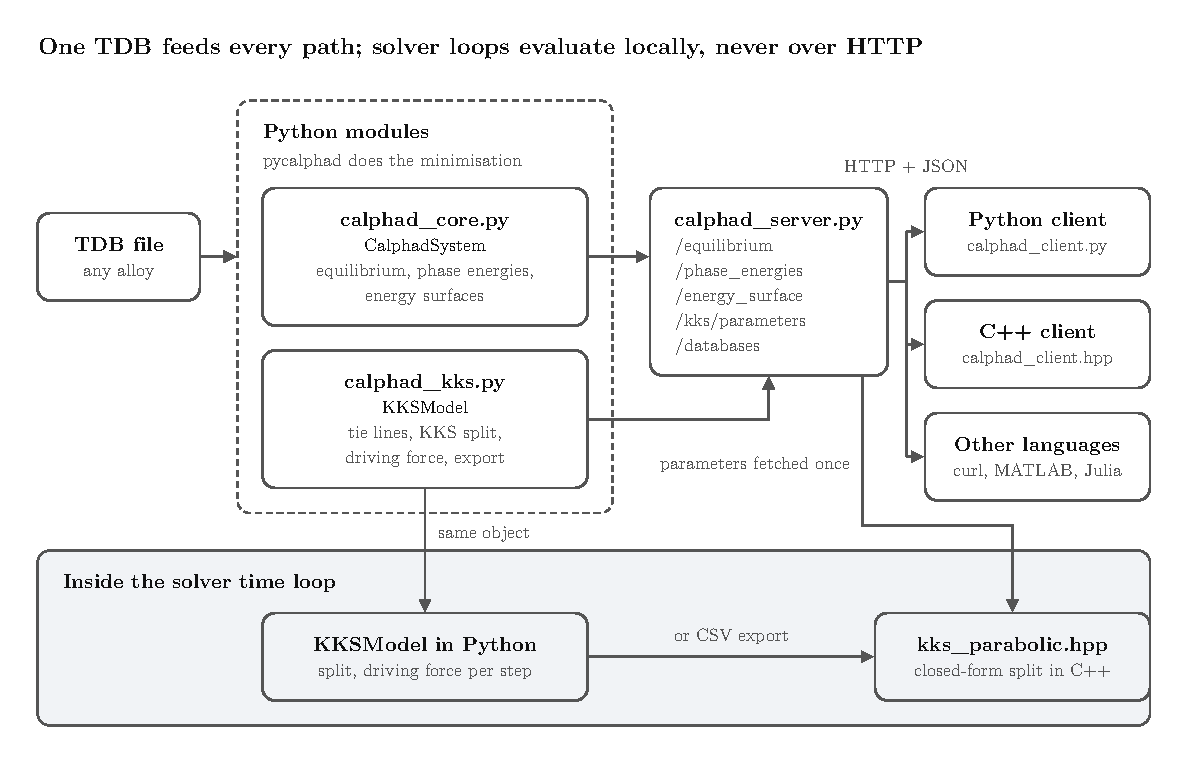
\includegraphics[width=1.00\textwidth]{architecture.pdf}
\caption{Framework architecture: database, Python modules, server, clients and the solver loop.}
\label{fig:architecture}
\end{figure}
Python codes import the modules directly; every other language goes through the server. Inside a time loop, both paths evaluate the KKS formulas locally from parameters fetched once.


\needspace{10\baselineskip}
\section*{2. Installation and quick start}
\addcontentsline{toc}{section}{2. Installation and quick start}
Install three Python packages, start the server with a database, and make a first call. The examples below all ask the same question: Cu--33Ni (at.\%) at 1500 K, which is 53\% liquid and 47\% FCC.


\needspace{7\baselineskip}
\subsection*{Requirements}
\addcontentsline{toc}{subsection}{Requirements}
\begingroup\small
\begin{longtable}{>{\raggedright\arraybackslash}p{0.216\linewidth}>{\raggedright\arraybackslash}p{0.458\linewidth}>{\raggedright\arraybackslash}p{0.247\linewidth}}
\toprule
\textbf{Component} & \textbf{Needs} & \textbf{Tested with} \\
\midrule
\endhead
Python core, KKS module, server & Python 3.10+, \texttt{pycalphad}, \texttt{fastapi}, \texttt{uvicorn} & Python 3.13, pycalphad 0.11.2 \\
Demo figures & \texttt{matplotlib} & --- \\
C++ client and KKS header & C++17 compiler, CMake 3.14+ & GCC on Linux \\
C++ HTTP client only & \texttt{httplib.\allowbreak{}h} and \texttt{json.\allowbreak{}hpp} (header-only; CMake downloads them on the first build) & cpp-httplib 0.18.3, nlohmann/json 3.11.3 \\
\bottomrule
\end{longtable}
\endgroup
\texttt{cpp/\allowbreak{}kks\_\allowbreak{}parabolic.\allowbreak{}hpp} has no dependencies at all.


\needspace{7\baselineskip}
\subsection*{Install and start}
\addcontentsline{toc}{subsection}{Install and start}
\begin{enumerate}
\item Unzip \texttt{calphad\_\allowbreak{}server.\allowbreak{}zip} and open a terminal in the \texttt{calphad\_\allowbreak{}server} folder.
\item Install the packages:
\end{enumerate}
\begin{lstlisting}[basicstyle={\footnotesize\ttfamily},language=bash]
pip install pycalphad fastapi uvicorn matplotlib
\end{lstlisting}
\begin{enumerate}
\setcounter{enumi}{2}
\item Optionally check the installation. The last line should read \texttt{all 28 cases passed}:
\end{enumerate}
\begin{lstlisting}[basicstyle={\footnotesize\ttfamily},language=bash]
python selftest.py
\end{lstlisting}
\begin{enumerate}
\setcounter{enumi}{3}
\item Start the server with one or more databases:
\end{enumerate}
\begin{lstlisting}[basicstyle={\footnotesize\ttfamily},language=bash]
python calphad_server.py --tdb cuni_cost507.tdb
\end{lstlisting}
\begin{enumerate}
\setcounter{enumi}{4}
\item Open http://127.0.0.1:8000/docs in a browser. Every endpoint can be tried there with a ``Try it out'' button.
\end{enumerate}

\needspace{7\baselineskip}
\subsection*{First call, four ways}
\addcontentsline{toc}{subsection}{First call, four ways}
\textbf{Python, no server} (fastest; use this inside Python codes):

\begin{lstlisting}[basicstyle={\footnotesize\ttfamily},language=Python]
from calphad_core import CalphadSystem

s = CalphadSystem.from_file("cuni_cost507.tdb")
r = s.equilibrium({"NI": 0.33}, T=1500, balance="CU")
for p in r["results"]["phases"]:
    print(p["phase"], round(p["fraction"], 4), round(p["composition"]["NI"], 4))
# LIQUID 0.5344 0.2703
# FCC_A1 0.4656 0.3985
\end{lstlisting}
\textbf{Python, through the server:}

\begin{lstlisting}[basicstyle={\footnotesize\ttfamily},language=Python]
from calphad_client import CalphadClient

c = CalphadClient("http://127.0.0.1:8000")
r = c.equilibrium({"NI": 0.33}, T=1500, balance="CU")
\end{lstlisting}
\textbf{curl} (or any HTTP tool):

\begin{lstlisting}[basicstyle={\footnotesize\ttfamily},language=bash]
curl -X POST http://127.0.0.1:8000/equilibrium \
     -H "Content-Type: application/json" \
     -d '{"composition": {"NI": 0.33}, "balance": "CU", "T": 1500}'
\end{lstlisting}
\textbf{C++:}

\begin{lstlisting}[basicstyle={\footnotesize\ttfamily},language=bash]
cd cpp
cmake -S . -B build && cmake --build build
./build/calphad_example 127.0.0.1 8000
\end{lstlisting}
When only one database is loaded, requests may leave out \texttt{\textquotedbl{}db\textquotedbl{}}. With several loaded, every request must name one (section 4).


\needspace{10\baselineskip}
\section*{3. Conventions}
\addcontentsline{toc}{section}{3. Conventions}
Compositions are mole fractions and energies are J per mole of atoms, relative to the database's reference state, unless a field says otherwise. T is in K and P in Pa.


\needspace{7\baselineskip}
\subsection*{Units}
\addcontentsline{toc}{subsection}{Units}
\begingroup\small
\begin{longtable}{>{\raggedright\arraybackslash}p{0.271\linewidth}>{\raggedright\arraybackslash}p{0.239\linewidth}>{\raggedright\arraybackslash}p{0.411\linewidth}}
\toprule
\textbf{Quantity} & \textbf{Unit} & \textbf{Notes} \\
\midrule
\endhead
Temperature \texttt{T} & K &  \\
Pressure \texttt{P} & Pa & Default 101325 \\
Compositions in results & mole fraction & \texttt{composition\_\allowbreak{}wt} gives mass fractions \\
Phase \texttt{fraction} & fraction of the total moles of atoms & Sums to 1 over the stable phases \\
\texttt{GM}, \texttt{GM\_\allowbreak{}system}, chemical potentials & J/mol of atoms & Relative to the database reference state \\
KKS diffusion potential \texttt{mu} & J/mol & dG/dc = \(\mu_{\mathrm{solute}}\) \(-\) \(\mu_{\mathrm{solvent}}\) \\
KKS driving force & J/m\(^{3}\) by default & J/mol divided by \texttt{Vm}; \texttt{per\_\allowbreak{}volume=False} gives J/mol \\
Molar volume \texttt{Vm} & m\(^{3}\)/mol & You supply it (for example 7.0\(\times\)10\(^{-6}\) for Ni alloys) \\
\bottomrule
\end{longtable}
\endgroup

\needspace{7\baselineskip}
\subsection*{Specifying an alloy}
\addcontentsline{toc}{subsection}{Specifying an alloy}
APIs 1 and 2 take the same alloy fields:

\begingroup\small
\begin{longtable}{>{\raggedright\arraybackslash}p{0.161\linewidth}>{\raggedright\arraybackslash}p{0.148\linewidth}>{\raggedright\arraybackslash}p{0.121\linewidth}>{\raggedright\arraybackslash}p{0.464\linewidth}}
\toprule
\textbf{Field} & \textbf{Type} & \textbf{Default} & \textbf{Meaning} \\
\midrule
\endhead
\texttt{composition} & object, element \(\rightarrow\) amount & required & Element names are case-insensitive \\
\texttt{units} & string & \texttt{mole\_\allowbreak{}fraction} & \texttt{mole\_\allowbreak{}fraction}, \texttt{atomic\_\allowbreak{}percent}, \texttt{weight\_\allowbreak{}fraction} or \texttt{weight\_\allowbreak{}percent} \\
\texttt{balance} & string & none & Element that takes up the remainder; any value given for it is ignored \\
\texttt{P} & number & 101325 & Pressure in Pa \\
\texttt{phases} & list of strings & all & Restrict the candidate phases \\
\bottomrule
\end{longtable}
\endgroup
Without \texttt{balance}, the amounts must sum to 1 (or 100 for percent units) within 10\(^{-6}\). Weight units are converted with the database's atomic masses. Only the elements you name take part in the calculation, so a large multicomponent database can be used for any subsystem.

\begin{lstlisting}[basicstyle={\footnotesize\ttfamily}]
{"composition": {"NI": 0.33}, "balance": "CU"}
{"composition": {"CU": 0.67, "NI": 0.33}}
{"composition": {"NI": 30}, "units": "weight_percent", "balance": "CU"}
{"composition": {"AL": 20, "CR": 10}, "units": "atomic_percent", "balance": "NI"}
\end{lstlisting}
The first two lines are the same alloy. The third, Cu--30Ni by weight, becomes \(x_{\mathrm{Ni}}\) = 0.31696; the result's \texttt{alloy} field always echoes the mole fractions actually used.


\needspace{7\baselineskip}
\subsection*{Energy reference}
\addcontentsline{toc}{subsection}{Energy reference}
Energies are relative to the database's reference state, usually SER: the pure elements in their stable structure at 298.15 K and 1 bar. An absolute value such as \(-\)87 035 J/mol means nothing on its own. Differences between phases, compositions and temperatures are physical. Never mix energies from two different databases.


\needspace{7\baselineskip}
\subsection*{Phase names and order/disorder phases}
\addcontentsline{toc}{subsection}{Phase names and order/disorder phases}
\begin{itemize}
\item Phase names are exactly as in the TDB, in upper case.
\item Many databases describe an ordered phase and its disordered parent as one phase: \texttt{FCC\_\allowbreak{}L12} covers both \(\gamma '\) and \(\gamma\), and \texttt{BCC\_\allowbreak{}B2} covers both B2 and A2. pycalphad calculates with the ordered one only, so disordered \(\gamma\) comes back named \texttt{FCC\_\allowbreak{}L12}.
\item Each phase result therefore carries \texttt{state} (\texttt{\textquotedbl{}ordered\textquotedbl{}}, \texttt{\textquotedbl{}disordered\textquotedbl{}} or \texttt{null} for phases that cannot order) and \texttt{equivalent\_\allowbreak{}to} (the phase it really is). \texttt{\{\textquotedbl{}phase\textquotedbl{}: \textquotedbl{}FCC\_\allowbreak{}L12\textquotedbl{},\allowbreak{} \textquotedbl{}state\textquotedbl{}: \textquotedbl{}disordered\textquotedbl{},\allowbreak{} \textquotedbl{}equivalent\_\allowbreak{}to\textquotedbl{}: \textquotedbl{}FCC\_\allowbreak{}A1\textquotedbl{}\}} is \(\gamma\).
\item \texttt{composition\_\allowbreak{}set} numbers repeats of one phase. A \texttt{2} means a second instance: a miscibility gap, or ordered and disordered states side by side, such as \(\gamma\) + \(\gamma '\). API 2 lists such repeats as \texttt{\textquotedbl{}FCC\_\allowbreak{}L12\#2\textquotedbl{}}.
\item By default every phase that can form from the named elements is a candidate. When both members of an order/disorder pair qualify, the ordered one is kept. Each result's \texttt{candidate\_\allowbreak{}phases} shows the list used: asking Ni--Al for \texttt{[\textquotedbl{}FCC\_\allowbreak{}A1\textquotedbl{},\allowbreak{} \textquotedbl{}BCC\_\allowbreak{}B2\textquotedbl{},\allowbreak{} \textquotedbl{}BCC\_\allowbreak{}A2\textquotedbl{},\allowbreak{} \textquotedbl{}LIQUID\textquotedbl{}]} gives \texttt{[\textquotedbl{}BCC\_\allowbreak{}B2\textquotedbl{},\allowbreak{} \textquotedbl{}FCC\_\allowbreak{}A1\textquotedbl{},\allowbreak{} \textquotedbl{}LIQUID\textquotedbl{}]}.
\item \texttt{GET /\allowbreak{}databases/\allowbreak{}\{db\}} shows each phase's sublattices and any \texttt{order\_\allowbreak{}disorder\_\allowbreak{}pair}.
\end{itemize}

\needspace{7\baselineskip}
\subsection*{Missing values}
\addcontentsline{toc}{subsection}{Missing values}
JSON has no NaN, so an undefined number is \texttt{null}. Example: the Gibbs energy of a stoichiometric compound such as \texttt{AL3NI1} at a composition it cannot reach.


\needspace{7\baselineskip}
\subsection*{Errors}
\addcontentsline{toc}{subsection}{Errors}
\begingroup\small
\begin{longtable}{>{\raggedright\arraybackslash}p{0.094\linewidth}>{\raggedright\arraybackslash}p{0.234\linewidth}>{\raggedright\arraybackslash}p{0.592\linewidth}}
\toprule
\textbf{HTTP status} & \textbf{Cause} & \textbf{Example \texttt{detail}} \\
\midrule
\endhead
400 & Bad input & \texttt{Unknown element(s) [\textquotesingle{}FE\textquotesingle{}].\allowbreak{} Database has [\textquotesingle{}CU\textquotesingle{},\allowbreak{} \textquotesingle{}NI\textquotesingle{}].\allowbreak{}} \\
400 & Composition does not add up & \texttt{Composition sums to 0.\allowbreak{}3,\allowbreak{} not 1.\allowbreak{} Give all elements or name a \textquotesingle{}balance\textquotesingle{} element.\allowbreak{}} \\
400 & Several databases loaded, no \texttt{db} given & \texttt{Several databases loaded [\textquotesingle{}alcrni\textquotesingle{},\allowbreak{} \textquotesingle{}alni\_\allowbreak{}dupin\_\allowbreak{}2001\textquotesingle{},\allowbreak{} \textquotesingle{}cuni\_\allowbreak{}cost507\textquotesingle{}]; say which with \textquotesingle{}db\textquotesingle{}.\allowbreak{}} \\
400 & Request too large & \texttt{501501 grid points for 3 elements at step=0.\allowbreak{}001; increase step or max\_\allowbreak{}points (200000).\allowbreak{}} \\
404 & Database not loaded & \texttt{Database \textquotesingle{}cuni\textquotesingle{} not loaded.\allowbreak{} Loaded: [.\allowbreak{}.\allowbreak{}.\allowbreak{}]} \\
422 & Missing or wrongly typed field & \texttt{\{\textquotedbl{}type\textquotedbl{}: \textquotedbl{}missing\textquotedbl{},\allowbreak{} \textquotedbl{}loc\textquotedbl{}: [\textquotedbl{}body\textquotedbl{},\allowbreak{} \textquotedbl{}T\textquotedbl{}],\allowbreak{} \textquotedbl{}msg\textquotedbl{}: \textquotedbl{}Field required\textquotedbl{}\}} \\
500 & pycalphad failed & \texttt{\textless{}ExceptionType\textgreater{}: \textless{}message\textgreater{}} \\
\bottomrule
\end{longtable}
\endgroup
In Python, bad input raises \texttt{CalphadError} (a \texttt{ValueError}). The Python client raises \texttt{CalphadServerError(\textquotedbl{}HTTP 400: .\allowbreak{}.\allowbreak{}.\allowbreak{}\textquotedbl{})}; the C++ client throws \texttt{std::runtime\_\allowbreak{}error} with the same text.


\needspace{10\baselineskip}
\section*{4. Server and database management}
\addcontentsline{toc}{section}{4. Server and database management}
The server holds any number of databases in memory, each under a name, and every calculation request says which one to use.


\needspace{7\baselineskip}
\subsection*{Starting the server}
\addcontentsline{toc}{subsection}{Starting the server}
\begin{lstlisting}[basicstyle={\footnotesize\ttfamily},language=bash]
python calphad_server.py --tdb FILE [--tdb FILE ...] [--host HOST] [--port PORT]
\end{lstlisting}
\begingroup\small
\begin{longtable}{>{\raggedright\arraybackslash}p{0.094\linewidth}>{\raggedright\arraybackslash}p{0.108\linewidth}>{\raggedright\arraybackslash}p{0.719\linewidth}}
\toprule
\textbf{Option} & \textbf{Default} & \textbf{Meaning} \\
\midrule
\endhead
\texttt{-{}-{}tdb} & none & TDB file to load; repeat for several. Registered under its file name without \texttt{.\allowbreak{}tdb} \\
\texttt{-{}-{}host} & \texttt{127.\allowbreak{}0.\allowbreak{}0.\allowbreak{}1} & Only this machine can connect. \texttt{0.\allowbreak{}0.\allowbreak{}0.\allowbreak{}0} opens it to your network; there is no authentication, so only do that on a trusted network \\
\texttt{-{}-{}port} & \texttt{8000} & TCP port \\
\bottomrule
\end{longtable}
\endgroup
\begin{lstlisting}[basicstyle={\scriptsize\ttfamily},language=bash]
python calphad_server.py --tdb cuni_cost507.tdb --tdb alni_dupin_2001.tdb --tdb alcrni.tdb
\end{lstlisting}
Leave it running in its own terminal. Databases added later over HTTP last until the server stops.


\needspace{7\baselineskip}
\subsection*{Endpoints for databases}
\addcontentsline{toc}{subsection}{Endpoints for databases}
\begingroup\small
\begin{longtable}{>{\raggedright\arraybackslash}p{0.177\linewidth}>{\raggedright\arraybackslash}p{0.185\linewidth}>{\raggedright\arraybackslash}p{0.558\linewidth}}
\toprule
\textbf{Method and path} & \textbf{Body} & \textbf{Returns} \\
\midrule
\endhead
\texttt{GET /\allowbreak{}health} & --- & \texttt{\{\textquotedbl{}status\textquotedbl{}: \textquotedbl{}ok\textquotedbl{},\allowbreak{} \textquotedbl{}databases\textquotedbl{}: [.\allowbreak{}.\allowbreak{}.\allowbreak{}]\}} \\
\texttt{GET /\allowbreak{}databases} & --- & Each loaded database with its elements and phases \\
\texttt{POST /\allowbreak{}databases} & \texttt{path} or \texttt{tdb\_\allowbreak{}text}, optional \texttt{name} & The new database's full description \\
\texttt{GET /\allowbreak{}databases/\allowbreak{}\{db\}} & --- & Elements, atomic masses, phases, sublattices, order/disorder pairs \\
\texttt{GET /\allowbreak{}docs} & --- & Interactive documentation in the browser \\
\texttt{GET /\allowbreak{}openapi.\allowbreak{}json} & --- & Machine-readable description of every endpoint \\
\bottomrule
\end{longtable}
\endgroup

\needspace{7\baselineskip}
\subsection*{Example: list what is loaded}
\addcontentsline{toc}{subsection}{Example: list what is loaded}
\begin{lstlisting}[basicstyle={\footnotesize\ttfamily},language=bash]
curl http://127.0.0.1:8000/databases
\end{lstlisting}
\begin{lstlisting}[basicstyle={\scriptsize\ttfamily}]
{"cuni_cost507": {"elements": ["CU", "NI"], "phases": ["FCC_A1", "LIQUID"]},
 "alcrni": {"elements": ["AL", "CR", "NI"], "phases": ["B2", "BCC_A2", "FCC_A1", "L12_FCC", "LIQUID"]},
 "alni_dupin_2001": {"elements": ["AL", "NI"],
                     "phases": ["AL3NI1", "AL3NI2", "AL3NI5", "BCC_A2", "BCC_B2", "FCC_A1", "FCC_L12", "LIQUID"]}}
\end{lstlisting}

\needspace{7\baselineskip}
\subsection*{Example: load another database}
\addcontentsline{toc}{subsection}{Example: load another database}
By a path on the server's machine:

\begin{lstlisting}[basicstyle={\footnotesize\ttfamily},language=bash]
curl -X POST http://127.0.0.1:8000/databases -H "Content-Type: application/json" \
     -d '{"path": "/data/tdb/my_superalloy.tdb", "name": "ni_sx"}'
\end{lstlisting}
By sending the file's contents from your own machine (Python client):

\begin{lstlisting}[basicstyle={\footnotesize\ttfamily},language=Python]
c.upload_tdb("my_superalloy.tdb", name="ni_sx")
\end{lstlisting}
Loading under a name that already exists replaces that database.


\needspace{7\baselineskip}
\subsection*{Example: inspect a database}
\addcontentsline{toc}{subsection}{Example: inspect a database}
\begin{lstlisting}[basicstyle={\footnotesize\ttfamily},language=bash]
curl http://127.0.0.1:8000/databases/cuni_cost507
\end{lstlisting}
\begin{lstlisting}[basicstyle={\footnotesize\ttfamily}]
{"name": "cuni_cost507",
 "elements": ["CU", "NI"],
 "atomic_masses": {"CU": 63.546, "NI": 58.69},
 "phases": {
   "FCC_A1": {"site_ratios": [1.0, 1.0], "constituents": [["CU", "NI"], ["VA"]]},
   "LIQUID": {"site_ratios": [1.0], "constituents": [["CU", "NI"]]}}}
\end{lstlisting}
For \texttt{alni\_\allowbreak{}dupin\_\allowbreak{}2001}, the \texttt{FCC\_\allowbreak{}L12} entry also shows its order/disorder pair:

\begin{lstlisting}[basicstyle={\footnotesize\ttfamily}]
"FCC_L12": {"site_ratios": [0.75, 0.25, 1.0],
            "constituents": [["AL", "NI"], ["AL", "NI"], ["VA"]],
            "order_disorder_pair": {"ordered": "FCC_L12", "disordered": "FCC_A1"}}
\end{lstlisting}

\needspace{7\baselineskip}
\subsection*{The same without a server}
\addcontentsline{toc}{subsection}{The same without a server}
\begin{lstlisting}[basicstyle={\scriptsize\ttfamily},language=Python]
from calphad_core import CalphadSystem

s = CalphadSystem.from_file("alni_dupin_2001.tdb")     # or CalphadSystem.from_text(tdb_string, name="x")
s.name, s.elements, s.phases                             # 'alni_dupin_2001', ['AL', 'NI'], [...]
s.info()                                                 # same dict as GET /databases/{db}
\end{lstlisting}

\needspace{7\baselineskip}
\subsection*{Behaviour worth knowing}
\addcontentsline{toc}{subsection}{Behaviour worth knowing}
\begin{itemize}
\item The first calculation for a new set of elements and phases builds and compiles the thermodynamic models, which takes about a second. Later calls reuse them.
\item Calls on the same database are processed one at a time.
\item \texttt{/\allowbreak{}kks/\allowbreak{}parameters} keeps each KKS model it builds, so repeating a request with the same settings is fast.
\end{itemize}

\needspace{10\baselineskip}
\section*{5. API 1: Equilibrium --- \texttt{POST /\allowbreak{}equilibrium}}
\addcontentsline{toc}{section}{5. API 1: Equilibrium --- \texttt{POST /\allowbreak{}equilibrium}}
Given an alloy and a temperature, API 1 returns the stable phases, their fractions, their compositions and site fractions, and the system's chemical potentials. It is the ``read the phase diagram'' call.

\begingroup\small
\begin{longtable}{>{\raggedright\arraybackslash}p{0.155\linewidth}>{\raggedright\arraybackslash}p{0.792\linewidth}}
\toprule
\textbf{Access} & \textbf{Call} \\
\midrule
\endhead
HTTP & \texttt{POST /\allowbreak{}equilibrium} \\
Python, in-process & \texttt{CalphadSystem.\allowbreak{}equilibrium(composition,\allowbreak{} T,\allowbreak{} P=101325,\allowbreak{} phases=None,\allowbreak{} units=\textquotedbl{}mole\_\allowbreak{}fraction\textquotedbl{},\allowbreak{} balance=None,\allowbreak{} verify=True)} \\
Python client & \texttt{CalphadClient.\allowbreak{}equilibrium(composition,\allowbreak{} T,\allowbreak{} P=None,\allowbreak{} phases=None,\allowbreak{} units=None,\allowbreak{} balance=None,\allowbreak{} verify=None,\allowbreak{} db=None)} \\
C++ client & \texttt{CalphadClient::equilibrium(composition,\allowbreak{} T or vector\textless{}double\textgreater{},\allowbreak{} balance,\allowbreak{} extra)} \\
\bottomrule
\end{longtable}
\endgroup

\needspace{7\baselineskip}
\subsection*{Request}
\addcontentsline{toc}{subsection}{Request}
The alloy fields of section 3 (\texttt{composition}, \texttt{units}, \texttt{balance}, \texttt{P}, \texttt{phases}), plus:

\begingroup\small
\begin{longtable}{>{\raggedright\arraybackslash}p{0.094\linewidth}>{\raggedright\arraybackslash}p{0.211\linewidth}>{\raggedright\arraybackslash}p{0.156\linewidth}>{\raggedright\arraybackslash}p{0.432\linewidth}}
\toprule
\textbf{Field} & \textbf{Type} & \textbf{Default} & \textbf{Meaning} \\
\midrule
\endhead
\texttt{db} & string & the only database & Which database \\
\texttt{T} & number or list of numbers & required & K. A list returns one result per temperature \\
\texttt{verify} & boolean & \texttt{true} & Run the global-minimum check described below \\
\bottomrule
\end{longtable}
\endgroup

\needspace{7\baselineskip}
\subsection*{Response}
\addcontentsline{toc}{subsection}{Response}
\begingroup\small
\begin{longtable}{>{\raggedright\arraybackslash}p{0.305\linewidth}>{\raggedright\arraybackslash}p{0.642\linewidth}}
\toprule
\textbf{Field} & \textbf{Meaning} \\
\midrule
\endhead
\texttt{alloy} & Mole fractions actually used \\
\texttt{units\_\allowbreak{}in} & Units of the input composition \\
\texttt{candidate\_\allowbreak{}phases} & Phases considered \\
\texttt{results} & One result object, or a list of them when \texttt{T} was a list \\
\texttt{results.\allowbreak{}T}, \texttt{results.\allowbreak{}P} & Conditions \\
\texttt{results.\allowbreak{}converged} & \texttt{true} when every stable phase has a valid fraction \\
\texttt{results.\allowbreak{}GM\_\allowbreak{}system} & Gibbs energy of the equilibrium mixture, J/mol \\
\texttt{results.\allowbreak{}chemical\_\allowbreak{}potentials} & \(\mu\) of each element, J/mol: the common tangent plane \\
\texttt{results.\allowbreak{}phases[]} & Stable phases, largest fraction first \\
\texttt{results.\allowbreak{}stability\_\allowbreak{}check} & Outcome of the global-minimum check \\
\bottomrule
\end{longtable}
\endgroup
Each entry of \texttt{phases[]}:

\begingroup\small
\begin{longtable}{>{\raggedright\arraybackslash}p{0.219\linewidth}>{\raggedright\arraybackslash}p{0.728\linewidth}}
\toprule
\textbf{Field} & \textbf{Meaning} \\
\midrule
\endhead
\texttt{phase} & Phase name as in the database \\
\texttt{composition\_\allowbreak{}set} & 1, or 2+ for a repeat of the same phase \\
\texttt{state}, \texttt{equivalent\_\allowbreak{}to} & Order/disorder label (section 3) \\
\texttt{fraction} & Fraction of the total moles of atoms \\
\texttt{composition} & Mole fractions in this phase \\
\texttt{composition\_\allowbreak{}wt} & Mass fractions in this phase \\
\texttt{GM} & This phase's Gibbs energy at its own composition, J/mol (= \(\Sigma\) x\(_{i} \mu _{i}\)) \\
\texttt{site\_\allowbreak{}fractions} & One object per sublattice: species \(\rightarrow\) site fraction \\
\bottomrule
\end{longtable}
\endgroup

\needspace{7\baselineskip}
\subsection*{The stability check}
\addcontentsline{toc}{subsection}{The stability check}
pycalphad starts its minimiser from a sampled set of configurations. If the sample misses a phase's low-energy region, the answer is a local minimum. With \texttt{verify: true} (the default), every absent phase must have a driving force of at most 1 J/mol against the result's chemical potentials. If one is higher, the calculation is repeated with denser sampling: 2000, then 10 000 points per phase.

\begingroup\small
\begin{longtable}{>{\raggedright\arraybackslash}p{0.268\linewidth}>{\raggedright\arraybackslash}p{0.679\linewidth}}
\toprule
\textbf{Field} & \textbf{Meaning} \\
\midrule
\endhead
\texttt{verified} & \texttt{true} when no absent phase could lower the energy \\
\texttt{sampling\_\allowbreak{}density} & \texttt{\textquotedbl{}default\textquotedbl{}}, \texttt{2000} or \texttt{10000}: the density that passed \\
\texttt{driving\_\allowbreak{}forces\_\allowbreak{}absent\_\allowbreak{}phases} & Driving force of each absent phase, J/mol; all \(\le\) 0 when verified \\
\bottomrule
\end{longtable}
\endgroup
Why it matters: Ni--20Al--10Cr at 1600 K with \texttt{verify: false} returns L1\(_{2}\) 0.747 + liquid 0.253 at \(-\)118 162.44 J/mol. The check finds B2 with a positive driving force and re-solves: L1\(_{2}\) (disordered, so \(\gamma\)) 0.856 + B2 0.145 at \(-\)118 173.48 J/mol, 11 J/mol lower. \texttt{verified: false} means even the densest sampling left a phase with a positive driving force; treat that result with care. \texttt{verify: false} skips the check when speed matters more than certainty.


\needspace{7\baselineskip}
\subsection*{Example 5.1 --- one temperature}
\addcontentsline{toc}{subsection}{Example 5.1 --- one temperature}
Cu--33Ni (at.\%) at 1500 K.

\begin{lstlisting}[basicstyle={\footnotesize\ttfamily}]
{"db": "cuni_cost507", "composition": {"NI": 0.33}, "balance": "CU", "T": 1500}
\end{lstlisting}
\begin{lstlisting}[basicstyle={\footnotesize\ttfamily}]
{"alloy": {"NI": 0.33, "CU": 0.67},
 "units_in": "mole_fraction",
 "candidate_phases": ["FCC_A1", "LIQUID"],
 "results": {
   "T": 1500.0, "P": 101325.0, "converged": true,
   "GM_system": -87035.357,
   "chemical_potentials": {"CU": -86428.337, "NI": -88267.791},
   "phases": [
     {"phase": "LIQUID", "composition_set": 1, "state": null, "equivalent_to": null,
      "fraction": 0.534426,
      "composition": {"CU": 0.729662, "NI": 0.270338},
      "composition_wt": {"CU": 0.745054, "NI": 0.254946},
      "GM": -86925.612,
      "site_fractions": [{"CU": 0.729662, "NI": 0.270338}]},
     {"phase": "FCC_A1", "composition_set": 1, "state": null, "equivalent_to": null,
      "fraction": 0.465574,
      "composition": {"CU": 0.601515, "NI": 0.398485},
      "composition_wt": {"CU": 0.620407, "NI": 0.379593},
      "GM": -87161.332,
      "site_fractions": [{"CU": 0.601515, "NI": 0.398485}, {"VA": 1.0}]}],
   "stability_check": {"verified": true, "sampling_density": "default",
                       "driving_forces_absent_phases": {}}}}
\end{lstlisting}
(Numbers rounded to 6 significant digits here; the server returns full precision.) The two \texttt{composition} values are the tie-line ends at 1500 K, and the lever rule holds: 0.5344 \(\times\) 0.2703 + 0.4656 \(\times\) 0.3985 = 0.33.


\needspace{7\baselineskip}
\subsection*{Example 5.2 --- temperature sweep: solidus and liquidus}
\addcontentsline{toc}{subsection}{Example 5.2 --- temperature sweep: solidus and liquidus}
Ni--10Al from 1700 to 1725 K in one request.

\begin{lstlisting}[basicstyle={\footnotesize\ttfamily},language=Python]
r = s.equilibrium({"AL": 0.10}, [1700, 1717, 1718, 1719, 1720, 1725], balance="NI")
for res in r["results"]:
    print(res["T"], [(p["equivalent_to"] or p["phase"], round(p["fraction"], 4),
                      round(p["composition"]["AL"], 5)) for p in res["phases"]])
\end{lstlisting}
\begingroup\small
\begin{longtable}{>{\raggedright\arraybackslash}p{0.156\linewidth}>{\raggedright\arraybackslash}p{0.157\linewidth}>{\raggedright\arraybackslash}p{0.156\linewidth}>{\raggedright\arraybackslash}p{0.216\linewidth}>{\raggedright\arraybackslash}p{0.182\linewidth}}
\toprule
\textbf{T (K)} & \textbf{\(\gamma\) fraction} & \textbf{\(\gamma\) \(x_{\mathrm{Al}}\)} & \textbf{Liquid fraction} & \textbf{Liquid \(x_{\mathrm{Al}}\)} \\
\midrule
\endhead
1700 & 1.000 & 0.10000 & --- & --- \\
1717 & 1.000 & 0.10000 & --- & --- \\
1718 & 0.934 & 0.09937 & 0.066 & 0.10890 \\
1719 & 0.513 & 0.09568 & 0.487 & 0.10456 \\
1720 & --- & --- & 1.000 & 0.10000 \\
1725 & --- & --- & 1.000 & 0.10000 \\
\bottomrule
\end{longtable}
\endgroup
So the solidus of Ni--10Al lies between 1717 and 1718 K and the liquidus between 1719 and 1720 K (the demo in section 11 interpolates them as 1717.82 K and 1719.98 K). \(\gamma\) is reported as \texttt{FCC\_\allowbreak{}L12} with \texttt{state: \textquotedbl{}disordered\textquotedbl{}} and \texttt{equivalent\_\allowbreak{}to: \textquotedbl{}FCC\_\allowbreak{}A1\textquotedbl{}}. Each temperature is solved and checked separately; the list is a convenience, not a speed-up.


\needspace{7\baselineskip}
\subsection*{Example 5.3 --- weight percent}
\addcontentsline{toc}{subsection}{Example 5.3 --- weight percent}
Cu--30Ni by weight at 1500 K:

\begin{lstlisting}[basicstyle={\scriptsize\ttfamily}]
{"db": "cuni_cost507", "composition": {"NI": 30}, "units": "weight_percent", "balance": "CU", "T": 1500}
\end{lstlisting}
The response's \texttt{alloy} is \texttt{\{\textquotedbl{}NI\textquotedbl{}: 0.\allowbreak{}316955,\allowbreak{} \textquotedbl{}CU\textquotedbl{}: 0.\allowbreak{}683045\}}. Liquid is 0.6362 of the atoms and FCC 0.3638. The phase compositions are the same tie-line ends as in 5.1, since the temperature is the same: liquid 25.49 wt\% Ni and FCC 37.96 wt\% Ni in \texttt{composition\_\allowbreak{}wt}.


\needspace{7\baselineskip}
\subsection*{Example 5.4 --- restricting phases: metastable equilibrium}
\addcontentsline{toc}{subsection}{Example 5.4 --- restricting phases: metastable equilibrium}
Ni--25Al at 1000 K is single-phase \(\gamma '\). Leaving \(\gamma '\) out gives the metastable equilibrium without it, useful when \(\gamma '\) is kinetically suppressed, for example in rapid solidification.

\begin{lstlisting}[basicstyle={\footnotesize\ttfamily}]
{"db": "alni_dupin_2001", "composition": {"AL": 0.25}, "balance": "NI", "T": 1000,
 "phases": ["FCC_A1", "BCC_B2", "LIQUID"]}
\end{lstlisting}
\begingroup\small
\begin{longtable}{>{\raggedright\arraybackslash}p{0.285\linewidth}>{\raggedright\arraybackslash}p{0.662\linewidth}}
\toprule
\textbf{Request} & \textbf{Result} \\
\midrule
\endhead
All phases & \texttt{FCC\_\allowbreak{}L12} ordered (\(\gamma '\)), fraction 1.000 \\
\texttt{[\textquotedbl{}FCC\_\allowbreak{}A1\textquotedbl{},\allowbreak{} \textquotedbl{}BCC\_\allowbreak{}B2\textquotedbl{},\allowbreak{} \textquotedbl{}LIQUID\textquotedbl{}]} & \texttt{FCC\_\allowbreak{}A1} (\(\gamma\)) 0.520 at \(x_{\mathrm{Al}}\) 0.1939 + \texttt{BCC\_\allowbreak{}B2} ordered 0.480 at \(x_{\mathrm{Al}}\) 0.3109 \\
\bottomrule
\end{longtable}
\endgroup
Name the disordered phase (\texttt{FCC\_\allowbreak{}A1}) to exclude ordering; naming the ordered one (\texttt{FCC\_\allowbreak{}L12}) allows both states.


\needspace{7\baselineskip}
\subsection*{Example 5.5 --- ternary with ordered phases}
\addcontentsline{toc}{subsection}{Example 5.5 --- ternary with ordered phases}
Ni--20Al--10Cr (at.\%) at 1600 K in the \texttt{alcrni} database:

\begin{lstlisting}[basicstyle={\footnotesize\ttfamily}]
{"db": "alcrni", "composition": {"AL": 0.2, "CR": 0.1}, "balance": "NI", "T": 1600}
\end{lstlisting}
\begingroup\small
\begin{longtable}{>{\raggedright\arraybackslash}p{0.085\linewidth}>{\raggedright\arraybackslash}p{0.231\linewidth}>{\raggedright\arraybackslash}p{0.121\linewidth}>{\raggedright\arraybackslash}p{0.085\linewidth}>{\raggedright\arraybackslash}p{0.085\linewidth}>{\raggedright\arraybackslash}p{0.085\linewidth}>{\raggedright\arraybackslash}p{0.122\linewidth}}
\toprule
\textbf{Phase} & \textbf{\texttt{state} \(\rightarrow\) \texttt{equivalent\_\allowbreak{}to}} & \textbf{Fraction} & \textbf{\(x_{\mathrm{Al}}\)} & \textbf{\(x_{\mathrm{Cr}}\)} & \textbf{\(x_{\mathrm{Ni}}\)} & \textbf{GM (J/mol)} \\
\midrule
\endhead
\texttt{L12\_\allowbreak{}FCC} & disordered \(\rightarrow\) \texttt{FCC\_\allowbreak{}A1} & 0.8555 & 0.1857 & 0.1073 & 0.7070 & \(-\)116 858.1 \\
\texttt{B2} & ordered \(\rightarrow\) \texttt{B2} & 0.1445 & 0.2848 & 0.0567 & 0.6585 & \(-\)125 959.1 \\
\bottomrule
\end{longtable}
\endgroup
\texttt{GM\_\allowbreak{}system} is \(-\)118 173.48 J/mol and \texttt{stability\_\allowbreak{}check} shows \texttt{\textquotedbl{}sampling\_\allowbreak{}density\textquotedbl{}: 2000} with a liquid driving force of \(-\)26.09 J/mol. B2's \texttt{site\_\allowbreak{}fractions} show its ordering: Al fills 0.567 of the first sublattice but 0.002 of the second.


\needspace{7\baselineskip}
\subsection*{Example 5.6 --- one phase twice: \texorpdfstring{\(\gamma\)}{gamma} + \texorpdfstring{\(\gamma '\)}{gamma'} and a miscibility gap}
\addcontentsline{toc}{subsection}{Example 5.6 --- one phase twice: \texorpdfstring{\(\gamma\)}{gamma} + \texorpdfstring{\(\gamma '\)}{gamma'} and a miscibility gap}
Ni--20Al at 1000 K returns \texttt{FCC\_\allowbreak{}L12} twice:

\begingroup\small
\begin{longtable}{>{\raggedright\arraybackslash}p{0.112\linewidth}>{\raggedright\arraybackslash}p{0.161\linewidth}>{\raggedright\arraybackslash}p{0.360\linewidth}>{\raggedright\arraybackslash}p{0.121\linewidth}>{\raggedright\arraybackslash}p{0.112\linewidth}}
\toprule
\textbf{Phase} & \textbf{\texttt{composition\_\allowbreak{}set}} & \textbf{\texttt{state} \(\rightarrow\) \texttt{equivalent\_\allowbreak{}to}} & \textbf{Fraction} & \textbf{\(x_{\mathrm{Al}}\)} \\
\midrule
\endhead
\texttt{FCC\_\allowbreak{}L12} & 1 & ordered \(\rightarrow\) \texttt{FCC\_\allowbreak{}L12} (\(\gamma '\)) & 0.6697 & 0.2372 \\
\texttt{FCC\_\allowbreak{}L12} & 2 & disordered \(\rightarrow\) \texttt{FCC\_\allowbreak{}A1} (\(\gamma\)) & 0.3303 & 0.1246 \\
\bottomrule
\end{longtable}
\endgroup
Ni--40Al--20Cr at 1600 K (\texttt{alcrni}) does the same with B2: ordered B2 0.8268 (\(x_{\mathrm{Al}}\) 0.4642) and disordered B2, which is Cr-rich \(\alpha\) (\texttt{BCC\_\allowbreak{}A2}, \(x_{\mathrm{Cr}}\) 0.8811), 0.1732. Group results by \texttt{equivalent\_\allowbreak{}to or phase} to get physical phase names:

\begin{lstlisting}[basicstyle={\scriptsize\ttfamily},language=Python]
r = s.equilibrium({"AL": 0.20}, 1000, balance="NI")["results"]
for p in r["phases"]:
    print(p["equivalent_to"] or p["phase"], round(p["fraction"], 4), round(p["composition"]["AL"], 4))
# FCC_L12 0.6697 0.2372
# FCC_A1 0.3303 0.1246
\end{lstlisting}

\needspace{10\baselineskip}
\section*{6. API 2: Phase energies --- \texttt{POST /\allowbreak{}phase\_\allowbreak{}energies}}
\addcontentsline{toc}{section}{6. API 2: Phase energies --- \texttt{POST /\allowbreak{}phase\_\allowbreak{}energies}}
For one alloy composition and temperature, API 2 gives the Gibbs energy of every candidate phase at that composition, stable or not, with its own chemical potentials and its driving force. Use it for metastability, nucleation driving forces and free-energy inputs at a known composition.

\begingroup\small
\begin{longtable}{>{\raggedright\arraybackslash}p{0.155\linewidth}>{\raggedright\arraybackslash}p{0.792\linewidth}}
\toprule
\textbf{Access} & \textbf{Call} \\
\midrule
\endhead
HTTP & \texttt{POST /\allowbreak{}phase\_\allowbreak{}energies} \\
Python, in-process & \texttt{CalphadSystem.\allowbreak{}phase\_\allowbreak{}energies(composition,\allowbreak{} T,\allowbreak{} P=101325,\allowbreak{} phases=None,\allowbreak{} units=\textquotedbl{}mole\_\allowbreak{}fraction\textquotedbl{},\allowbreak{} balance=None)} \\
Python client & \texttt{CalphadClient.\allowbreak{}phase\_\allowbreak{}energies(composition,\allowbreak{} T,\allowbreak{} P=None,\allowbreak{} phases=None,\allowbreak{} units=None,\allowbreak{} balance=None,\allowbreak{} db=None)} \\
C++ client & \texttt{CalphadClient::phase\_\allowbreak{}energies(composition,\allowbreak{} T,\allowbreak{} balance,\allowbreak{} extra)} \\
\bottomrule
\end{longtable}
\endgroup

\needspace{7\baselineskip}
\subsection*{What it computes}
\addcontentsline{toc}{subsection}{What it computes}
Each phase is minimised on its own, as one homogeneous phase at the alloy composition. Its internal variables (sublattice occupancies, ordering) relax; its composition does not. pycalphad's \texttt{IsolatedPhase} does this. The framework also refines each phase from ordered and disordered starting configurations and keeps the lowest, because pycalphad alone returned disordered \(\gamma '\) for Ni--25Al at 1600 K, 355 J/mol too high.


\needspace{7\baselineskip}
\subsection*{Request}
\addcontentsline{toc}{subsection}{Request}
The alloy fields of section 3, plus \texttt{db} and \texttt{T} (a single number, K). The equilibrium used for comparison is always verified.


\needspace{7\baselineskip}
\subsection*{Response}
\addcontentsline{toc}{subsection}{Response}
\begingroup\small
\begin{longtable}{>{\raggedright\arraybackslash}p{0.193\linewidth}>{\raggedright\arraybackslash}p{0.754\linewidth}}
\toprule
\textbf{Field} & \textbf{Meaning} \\
\midrule
\endhead
\texttt{alloy}, \texttt{T}, \texttt{P} & Conditions \\
\texttt{GM\_\allowbreak{}equilibrium} & G of the equilibrium mixture at this composition, J/mol \\
\texttt{stable\_\allowbreak{}phases} & Equilibrium phases; repeats as \texttt{\textquotedbl{}FCC\_\allowbreak{}L12\#2\textquotedbl{}} \\
\texttt{stability\_\allowbreak{}check} & As in API 1 \\
\texttt{phases[]} & One entry per candidate phase, lowest \texttt{GM} first, unreachable phases last \\
\bottomrule
\end{longtable}
\endgroup
Each entry of \texttt{phases[]}:

\begingroup\small
\begin{longtable}{>{\raggedright\arraybackslash}p{0.243\linewidth}>{\raggedright\arraybackslash}p{0.704\linewidth}}
\toprule
\textbf{Field} & \textbf{Meaning} \\
\midrule
\endhead
\texttt{GM} & G of this phase alone at the alloy composition, J/mol; \texttt{null} if it cannot reach it \\
\texttt{chemical\_\allowbreak{}potentials} & This phase's tangent plane at this composition, J/mol per element \\
\texttt{state}, \texttt{equivalent\_\allowbreak{}to}, \texttt{site\_\allowbreak{}fractions} & As in API 1, for this phase's minimised state \\
\texttt{GM\_\allowbreak{}above\_\allowbreak{}equilibrium} & \texttt{GM \(-\) GM\_\allowbreak{}equilibrium}, \(\ge\) 0: the cost of forcing the whole alloy into this phase \\
\texttt{driving\_\allowbreak{}force} & J/mol, against the equilibrium chemical potentials: 0 for stable phases, negative for the rest \\
\texttt{splits\_\allowbreak{}if\_\allowbreak{}allowed} & Present when this phase on its own would rather separate into two compositions: \texttt{GM} of that split and its \texttt{composition\_\allowbreak{}sets} \\
\texttt{note} & Why \texttt{GM} is \texttt{null} \\
\bottomrule
\end{longtable}
\endgroup
\textbf{\texttt{GM\_\allowbreak{}above\_\allowbreak{}equilibrium}}\textbf{ versus }\textbf{\texttt{driving\_\allowbreak{}force}}\textbf{.} The first is measured at the alloy composition. The second is the largest gap between the equilibrium tangent plane and the phase's G curve over all the phase's compositions. A stable phase has \texttt{driving\_\allowbreak{}force} 0 even when its \texttt{GM\_\allowbreak{}above\_\allowbreak{}equilibrium} is positive, because a different composition of it touches the tangent. Use \texttt{driving\_\allowbreak{}force} for nucleation.

\textbf{Diffusion potentials.} In a binary A--B, \texttt{chemical\_\allowbreak{}potentials[B] \(-\) chemical\_\allowbreak{}potentials[A]} of a phase is dG/dc of that phase at this composition: the diffusion potential a KKS solver equates between phases.


\needspace{7\baselineskip}
\subsection*{Example 6.1 --- a two-phase alloy}
\addcontentsline{toc}{subsection}{Example 6.1 --- a two-phase alloy}
Cu--33Ni at 1500 K, where liquid and FCC coexist:

\begin{lstlisting}[basicstyle={\footnotesize\ttfamily}]
{"db": "cuni_cost507", "composition": {"NI": 0.33}, "balance": "CU", "T": 1500}
\end{lstlisting}
\begin{lstlisting}[basicstyle={\scriptsize\ttfamily}]
{"alloy": {"NI": 0.33, "CU": 0.67}, "T": 1500.0, "P": 101325.0,
 "GM_equilibrium": -87035.357,
 "stable_phases": ["LIQUID", "FCC_A1"],
 "stability_check": {"verified": true, "sampling_density": "default", "driving_forces_absent_phases": {}},
 "phases": [
   {"phase": "LIQUID", "GM": -86975.228,
    "chemical_potentials": {"CU": -87010.056, "NI": -86904.515},
    "state": null, "equivalent_to": null,
    "site_fractions": [{"CU": 0.67, "NI": 0.33}],
    "GM_above_equilibrium": 60.129, "driving_force": 0.0},
   {"phase": "FCC_A1", "GM": -86970.388,
    "chemical_potentials": {"CU": -85719.159, "NI": -89510.761},
    "state": null, "equivalent_to": null,
    "site_fractions": [{"CU": 0.67, "NI": 0.33}, {"VA": 1.0}],
    "GM_above_equilibrium": 64.969, "driving_force": 0.0}]}
\end{lstlisting}
Forcing the alloy to be all liquid costs 60.1 J/mol and all FCC 65.0 J/mol; the two-phase mixture is lower than either. The diffusion potentials at \(x_{\mathrm{Ni}}\) = 0.33 are 105.5 J/mol in the liquid and \(-\)3791.6 J/mol in FCC. They differ because \(x_{\mathrm{Ni}}\) = 0.33 is not on either tie-line end.


\needspace{7\baselineskip}
\subsection*{Example 6.2 --- an ordered phase and compounds}
\addcontentsline{toc}{subsection}{Example 6.2 --- an ordered phase and compounds}
Ni--25Al at 1600 K (\texttt{alni\_\allowbreak{}dupin\_\allowbreak{}2001}):

\begingroup\small
\begin{longtable}{>{\raggedright\arraybackslash}p{0.211\linewidth}>{\raggedright\arraybackslash}p{0.116\linewidth}>{\raggedright\arraybackslash}p{0.132\linewidth}>{\raggedright\arraybackslash}p{0.219\linewidth}>{\raggedright\arraybackslash}p{0.189\linewidth}}
\toprule
\textbf{Phase} & \textbf{\texttt{state}} & \textbf{GM (J/mol)} & \textbf{Above equilibrium (J/mol)} & \textbf{Driving force (J/mol)} \\
\midrule
\endhead
\texttt{FCC\_\allowbreak{}L12} & ordered (\(\gamma '\)) & \(-\)122 316.2 & 0.0 & 0.0 \\
\texttt{BCC\_\allowbreak{}B2} & ordered & \(-\)122 024.5 & 291.7 & \(-\)98.1 \\
\texttt{LIQUID} & --- & \(-\)121 793.5 & 522.7 & \(-\)522.4 \\
\texttt{AL3NI1}, \texttt{AL3NI2}, \texttt{AL3NI5} & --- & \texttt{null} & --- & --- \\
\bottomrule
\end{longtable}
\endgroup
\(\gamma '\) is stable. B2 at this composition is 291.7 J/mol above it, but a more Al-rich B2 comes within 98.1 J/mol of the tangent plane, which is the number that matters for whether B2 could nucleate. The three compounds are stoichiometric and cannot reach \(x_{\mathrm{Al}}\) = 0.25, so their \texttt{note} reads \texttt{phase cannot attain this composition (e.\allowbreak{}g.\allowbreak{} a stoichiometric compound)}.


\needspace{7\baselineskip}
\subsection*{Example 6.3 --- a phase that would rather split}
\addcontentsline{toc}{subsection}{Example 6.3 --- a phase that would rather split}
Ni--20Al at 1000 K is \(\gamma\) + \(\gamma '\), both described by \texttt{FCC\_\allowbreak{}L12}. As one homogeneous phase, \texttt{FCC\_\allowbreak{}L12} has GM = \(-\)74 334.4 J/mol, 122.7 J/mol above equilibrium. Allowed to separate, it splits into the equilibrium itself:

\begin{lstlisting}[basicstyle={\scriptsize\ttfamily}]
{"phase": "FCC_L12", "GM": -74334.4, "state": "ordered",
 "GM_above_equilibrium": 122.7, "driving_force": 0.0,
 "splits_if_allowed": {"GM": -74457.12,
   "composition_sets": [{"fraction": 0.6697, "composition": {"AL": 0.2372, "NI": 0.7628}},
                        {"fraction": 0.3303, "composition": {"AL": 0.1246, "NI": 0.8754}}]}}
\end{lstlisting}
\texttt{stable\_\allowbreak{}phases} is \texttt{[\textquotedbl{}FCC\_\allowbreak{}L12\textquotedbl{},\allowbreak{} \textquotedbl{}FCC\_\allowbreak{}L12\#2\textquotedbl{}]}. The other phases are far away: B2 2476.1 J/mol above (driving force \(-\)2475.3) and liquid 8007.5 J/mol above (driving force \(-\)7624.4).


\needspace{7\baselineskip}
\subsection*{Example 6.4 --- ranking phases by driving force}
\addcontentsline{toc}{subsection}{Example 6.4 --- ranking phases by driving force}
\begin{lstlisting}[basicstyle={\scriptsize\ttfamily},language=Python]
pe = s.phase_energies({"AL": 0.20}, 1000, balance="NI")
for p in pe["phases"]:
    if p["GM"] is None:
        continue
    print(f'{p["phase"]:8s} above eq {p["GM_above_equilibrium"]:8.1f}  driving force {p["driving_force"]:8.1f}')
# FCC_L12  above eq    122.7  driving force      0.0
# BCC_B2   above eq   2476.1  driving force  -2475.3
# LIQUID   above eq   8007.5  driving force  -7624.4
\end{lstlisting}

\needspace{10\baselineskip}
\section*{7. API 3: Energy surfaces --- \texttt{POST /\allowbreak{}energy\_\allowbreak{}surface}}
\addcontentsline{toc}{section}{7. API 3: Energy surfaces --- \texttt{POST /\allowbreak{}energy\_\allowbreak{}surface}}
At one temperature, API 3 returns G(x) of every candidate phase over the whole composition space: curves for a binary, surfaces for a ternary. Use it to plot free-energy diagrams, build lookup tables or fit your own free-energy functions.

\begingroup\small
\begin{longtable}{>{\raggedright\arraybackslash}p{0.155\linewidth}>{\raggedright\arraybackslash}p{0.792\linewidth}}
\toprule
\textbf{Access} & \textbf{Call} \\
\midrule
\endhead
HTTP & \texttt{POST /\allowbreak{}energy\_\allowbreak{}surface} \\
Python, in-process & \texttt{CalphadSystem.\allowbreak{}energy\_\allowbreak{}surface(T,\allowbreak{} P=101325,\allowbreak{} elements=None,\allowbreak{} phases=None,\allowbreak{} step=0.\allowbreak{}02,\allowbreak{} mode=\textquotedbl{}grid\textquotedbl{},\allowbreak{} pdens=500,\allowbreak{} max\_\allowbreak{}points=200000)} \\
Python client & \texttt{CalphadClient.\allowbreak{}energy\_\allowbreak{}surface(T,\allowbreak{} P=None,\allowbreak{} elements=None,\allowbreak{} phases=None,\allowbreak{} mode=None,\allowbreak{} step=None,\allowbreak{} pdens=None,\allowbreak{} max\_\allowbreak{}points=None,\allowbreak{} db=None)} \\
C++ client & \texttt{CalphadClient::energy\_\allowbreak{}surface(T,\allowbreak{} extra)} \\
\bottomrule
\end{longtable}
\endgroup

\needspace{7\baselineskip}
\subsection*{Request}
\addcontentsline{toc}{subsection}{Request}
\begingroup\small
\begin{longtable}{>{\raggedright\arraybackslash}p{0.121\linewidth}>{\raggedright\arraybackslash}p{0.189\linewidth}>{\raggedright\arraybackslash}p{0.152\linewidth}>{\raggedright\arraybackslash}p{0.433\linewidth}}
\toprule
\textbf{Field} & \textbf{Type} & \textbf{Default} & \textbf{Meaning} \\
\midrule
\endhead
\texttt{db} & string & the only database & Which database \\
\texttt{T} & number & required & K \\
\texttt{P} & number & 101325 & Pa \\
\texttt{elements} & list & all elements & A subsystem, for example \texttt{[\textquotedbl{}AL\textquotedbl{},\allowbreak{} \textquotedbl{}NI\textquotedbl{}]} of Al--Cr--Ni \\
\texttt{phases} & list & all & Restrict the phases \\
\texttt{mode} & \texttt{\textquotedbl{}grid\textquotedbl{}} or \texttt{\textquotedbl{}points\textquotedbl{}} & \texttt{\textquotedbl{}grid\textquotedbl{}} & See below \\
\texttt{step} & number, 0 < step \(\le\) 0.5 & 0.02 & Grid spacing in mole fraction \\
\texttt{pdens} & integer & 500 & Sampling density for phases with sublattices \\
\texttt{max\_\allowbreak{}points} & integer & 200 000 & Upper limit on points per phase \\
\bottomrule
\end{longtable}
\endgroup

\needspace{7\baselineskip}
\subsection*{The two modes}
\addcontentsline{toc}{subsection}{The two modes}
\textbf{\texttt{grid}} evaluates each phase on a regular composition grid that includes the pure elements. A binary at \texttt{step} 0.01 has 101 nodes; a ternary has 1326 at 0.02 and 5151 at 0.01.

\begin{itemize}
\item Substitutional phases (all elements on one sublattice, any other sublattice vacancies only: \texttt{LIQUID}, \texttt{FCC\_\allowbreak{}A1}, \texttt{BCC\_\allowbreak{}A2} and the like) get the exact G at each node: \texttt{\textquotedbl{}approximate\textquotedbl{}: false}.
\item Phases with sublattices (ordered phases, compounds) have internal configurations as well as a composition. pycalphad samples them and the lowest-energy sample in each grid cell is kept: \texttt{\textquotedbl{}approximate\textquotedbl{}: true}. Its \texttt{X} is that sample's own composition, within half a step of the node, not the node itself. Raise \texttt{pdens} for more samples.
\item Stoichiometric compounds only cover the cells they can reach, so their \texttt{n\_\allowbreak{}points} is small.
\end{itemize}
\textbf{\texttt{points}} returns every sampled configuration, including higher-energy orderings, thinned at random to \texttt{max\_\allowbreak{}points} if needed. Use it to see all branches of an ordered phase.


\needspace{7\baselineskip}
\subsection*{Response}
\addcontentsline{toc}{subsection}{Response}
\begingroup\small
\begin{longtable}{>{\raggedright\arraybackslash}p{0.235\linewidth}>{\raggedright\arraybackslash}p{0.712\linewidth}}
\toprule
\textbf{Field} & \textbf{Meaning} \\
\midrule
\endhead
\texttt{T}, \texttt{P} & Conditions \\
\texttt{elements} & Element order of the columns of \texttt{X} (alphabetical) \\
\texttt{mode}, \texttt{step} & As requested (\texttt{step} is \texttt{null} in points mode) \\
\texttt{phases[].\allowbreak{}phase} & Phase name \\
\texttt{phases[].\allowbreak{}n\_\allowbreak{}points} & Number of points \\
\texttt{phases[].\allowbreak{}approximate} & \texttt{true} for sampled phases in grid mode \\
\texttt{phases[].\allowbreak{}X} & List of compositions; each row is mole fractions in \texttt{elements} order \\
\texttt{phases[].\allowbreak{}GM} & G at each row of \texttt{X}, J/mol \\
\bottomrule
\end{longtable}
\endgroup

\needspace{7\baselineskip}
\subsection*{Example 7.1 --- binary free-energy curves}
\addcontentsline{toc}{subsection}{Example 7.1 --- binary free-energy curves}
Cu--Ni at 1500 K: 101 exact points for each of \texttt{FCC\_\allowbreak{}A1} and \texttt{LIQUID}.

\begin{lstlisting}[basicstyle={\footnotesize\ttfamily}]
{"db": "cuni_cost507", "T": 1500, "step": 0.01}
\end{lstlisting}
The first rows of \texttt{FCC\_\allowbreak{}A1} are \texttt{X: [[0.\allowbreak{}0,\allowbreak{} 1.\allowbreak{}0],\allowbreak{} [0.\allowbreak{}01,\allowbreak{} 0.\allowbreak{}99],\allowbreak{} .\allowbreak{}.\allowbreak{}.\allowbreak{}]} (columns Cu, Ni, so pure Ni first) and \texttt{GM: [-{}81682.\allowbreak{}09,\allowbreak{} -{}82248.\allowbreak{}35,\allowbreak{} .\allowbreak{}.\allowbreak{}.\allowbreak{}]}. Plotting:

\begin{lstlisting}[basicstyle={\scriptsize\ttfamily},language=Python]
import numpy as np
import matplotlib.pyplot as plt

surf = s.energy_surface(T=1500, step=0.01)      # or c.energy_surface(T=1500, step=0.01, db="cuni_cost507")
i_ni = surf["elements"].index("NI")
for ph in surf["phases"]:
    X = np.array(ph["X"])
    G = np.array(ph["GM"], dtype=float)
    order = np.argsort(X[:, i_ni])
    plt.plot(X[order, i_ni], G[order] / 1000, label=ph["phase"])
plt.xlabel("x_Ni")
plt.ylabel("G (kJ/mol)")
plt.legend()
plt.show()
\end{lstlisting}

\needspace{7\baselineskip}
\subsection*{Example 7.2 --- ternary surface on a Gibbs triangle}
\addcontentsline{toc}{subsection}{Example 7.2 --- ternary surface on a Gibbs triangle}
Al--Cr--Ni at 1273 K, \texttt{step} 0.02: 1326 exact points for \texttt{LIQUID}; \texttt{B2} and \texttt{L12\_\allowbreak{}FCC} are marked approximate.

\begin{lstlisting}[basicstyle={\scriptsize\ttfamily},language=Python]
surf = t.energy_surface(T=1273, step=0.02)        # t = CalphadSystem.from_file("alcrni.tdb")
el = surf["elements"]                              # ['AL', 'CR', 'NI']
liq = next(p for p in surf["phases"] if p["phase"] == "LIQUID")
X = np.array(liq["X"])
G = np.array(liq["GM"], dtype=float)
xa, xc = X[:, el.index("AL")], X[:, el.index("CR")]
px = xc + 0.5 * xa                                 # Ni bottom-left, Cr bottom-right, Al top
py = np.sqrt(3) / 2 * xa
plt.tricontourf(px, py, G / 1000, levels=20)
plt.colorbar(label="G of LIQUID (kJ/mol)")
plt.gca().set_aspect("equal")
plt.axis("off")
plt.show()
\end{lstlisting}

\needspace{7\baselineskip}
\subsection*{Example 7.3 --- a binary subsystem of a larger database}
\addcontentsline{toc}{subsection}{Example 7.3 --- a binary subsystem of a larger database}
\begin{lstlisting}[basicstyle={\footnotesize\ttfamily}]
{"db": "alcrni", "T": 1273, "elements": ["AL", "NI"], "step": 0.02}
\end{lstlisting}
Returns 51 points per phase along the Al--Ni edge; Cr is left out of the calculation entirely.


\needspace{7\baselineskip}
\subsection*{Example 7.4 --- the lowest single phase at each composition}
\addcontentsline{toc}{subsection}{Example 7.4 --- the lowest single phase at each composition}
Because sampled phases are not exactly on the nodes, compare phases by grid cell, not by exact composition:

\begin{lstlisting}[basicstyle={\scriptsize\ttfamily},language=Python]
step = 0.02
surf = s.energy_surface(T=1000, step=step, phases=["FCC_L12", "BCC_B2", "LIQUID"])   # Ni-Al
i_al = surf["elements"].index("AL")
lowest = {}                                   # grid cell -> (phase, G)
for ph in surf["phases"]:
    for x, g in zip(ph["X"], ph["GM"]):
        cell = round(x[i_al] / step)
        if g is not None and (cell not in lowest or g < lowest[cell][1]):
            lowest[cell] = (ph["phase"], g)
for cell in range(0, 46, 5):
    print(f"x_Al = {cell * step:.2f}: {lowest[cell][0]}")
# x_Al = 0.00 (*@\ldots{}@*) 0.30: FCC_L12    x_Al = 0.40 (*@\ldots{}@*) 0.80: BCC_B2    x_Al = 0.90: LIQUID
\end{lstlisting}
This compares single phases, not mixtures; for which phases coexist, use API 1. Within one cell, a sampled phase sits up to half a step from the node, so near the pure-element ends, where G is steep, use API 2 for an exact comparison at one composition.


\needspace{7\baselineskip}
\subsection*{Example 7.5 --- every sampled configuration}
\addcontentsline{toc}{subsection}{Example 7.5 --- every sampled configuration}
\begin{lstlisting}[basicstyle={\scriptsize\ttfamily}]
{"db": "alni_dupin_2001", "T": 1000, "mode": "points", "pdens": 200, "phases": ["FCC_L12", "LIQUID"]}
\end{lstlisting}
Returns 1604 points for \texttt{FCC\_\allowbreak{}L12} (ordered and disordered configurations together) and 402 for \texttt{LIQUID}. Plotted as a scatter of G against \(x_{\mathrm{Al}}\), the lower edge of the \texttt{FCC\_\allowbreak{}L12} cloud is its stable branch.


\needspace{7\baselineskip}
\subsection*{Speed}
\addcontentsline{toc}{subsection}{Speed}
Grid mode is fast: Cu--Ni at \texttt{step} 0.01 takes a few milliseconds, Al--Cr--Ni at \texttt{step} 0.05 about 0.07 s. Responses grow with the number of points, so prefer \texttt{step} \(\ge\) 0.01 for ternaries over HTTP.


\needspace{10\baselineskip}
\section*{8. KKS module --- \texttt{calphad\_\allowbreak{}kks.\allowbreak{}py}}
\addcontentsline{toc}{section}{8. KKS module --- \texttt{calphad\_\allowbreak{}kks.\allowbreak{}py}}
\texttt{KKSModel} turns a TDB into what a KKS phase-field solver needs for a binary alloy with two phases: each phase's free energy, the equilibrium tie lines, the KKS composition split at every grid point, and the driving force. Inputs are NumPy arrays of any shape, and T may be a field.


\needspace{7\baselineskip}
\subsection*{8.1 The model in brief}
\addcontentsline{toc}{subsection}{8.1 The model in brief}
At every point, the overall composition c is split into the two phase compositions \(c_{a}\) and \(c_{b}\) so that both the mixture rule and equal diffusion potential hold:

\begin{equation*}
c = h(\phi)\,c_a + \bigl(1 - h(\phi)\bigr)\,c_b, \qquad \frac{\partial f_a}{\partial c}(c_a) = \frac{\partial f_b}{\partial c}(c_b) = \tilde\mu
\end{equation*}
The phase field and the composition then evolve as:

\begin{equation*}
\frac{\partial \phi}{\partial t} = M\Bigl[\varepsilon^2 \nabla^2\phi - W g'(\phi) - h'(\phi)\,\bigl(f_a(c_a) - f_b(c_b) - \tilde\mu\,(c_a - c_b)\bigr)\Bigr]
\end{equation*}
\begin{equation*}
\frac{\partial c}{\partial t} = \nabla\cdot\Bigl[D(\phi)\bigl(h\,\nabla c_a + (1-h)\,\nabla c_b\bigr)\Bigr]
\end{equation*}
with h(\(\phi\)) = \(\phi ^{3}\)(6\(\phi ^{2}\) \(-\) 15\(\phi\) + 10) and g(\(\phi\)) = \(\phi ^{2}\)(1 \(-\) \(\phi\))\(^{2}\). \(\phi\) = 1 is \texttt{phase\_\allowbreak{}a}, f = G / Vm in J/m\(^{3}\), and c is the mole fraction of the solute. The interface energy \(\sigma\) and width 2\(\lambda\) (\(\phi\) from 0.1 to 0.9) set the gradient and barrier coefficients (Kim, Kim \& Suzuki, Phys. Rev. E 60, 7186, 1999):

\begin{equation*}
\sigma = \frac{\varepsilon\sqrt{W}}{3\sqrt{2}}, \qquad 2\lambda = \frac{2.2\sqrt{2}\,\varepsilon}{\sqrt{W}}
\end{equation*}
The module provides everything inside the square brackets except \(\varepsilon ^{2} \nabla ^{2} \phi\), which is your solver's stencil. M and D(\(\phi\)) are yours to choose.


\needspace{7\baselineskip}
\subsection*{8.2 Constructing a model}
\addcontentsline{toc}{subsection}{8.2 Constructing a model}
\begin{lstlisting}[basicstyle={\scriptsize\ttfamily},language=Python]
KKSModel(system, solute, phase_a, phase_b, mode="exact", Vm=None, c_alloy=None, T=None,
         solvent=None, reference=None, n_c=201, c_range=(1e-4, 1 - 1e-4), branches=None)

KKSModel.from_tdb(path, solute, phase_a, phase_b, **same_keywords)
\end{lstlisting}
\begingroup\small
\begin{longtable}{>{\raggedright\arraybackslash}p{0.134\linewidth}>{\raggedright\arraybackslash}p{0.136\linewidth}>{\raggedright\arraybackslash}p{0.650\linewidth}}
\toprule
\textbf{Parameter} & \textbf{Default} & \textbf{Meaning} \\
\midrule
\endhead
\texttt{system} & required & A \texttt{CalphadSystem} (or use \texttt{from\_\allowbreak{}tdb} with a file path) \\
\texttt{solute} & required & Element B; c = \(x_{B}\) \\
\texttt{phase\_\allowbreak{}a} & required & Phase at \(\phi\) = 1, usually the solid (\texttt{\textquotedbl{}FCC\_\allowbreak{}A1\textquotedbl{}}) \\
\texttt{phase\_\allowbreak{}b} & required & Phase at \(\phi\) = 0, usually \texttt{\textquotedbl{}LIQUID\textquotedbl{}} \\
\texttt{mode} & \texttt{\textquotedbl{}exact\textquotedbl{}} & \texttt{\textquotedbl{}exact\textquotedbl{}}, \texttt{\textquotedbl{}table\textquotedbl{}} or \texttt{\textquotedbl{}parabolic\textquotedbl{}} (8.3) \\
\texttt{Vm} & \texttt{None} & Molar volume, m\(^{3}\)/mol; needed for anything per volume \\
\texttt{c\_\allowbreak{}alloy} & \texttt{None} & Nominal composition; picks the right two-phase field when the two phases meet more than once \\
\texttt{T} & \texttt{None} & Temperatures for \texttt{table} and \texttt{parabolic}: a list, or a tuple \texttt{(Tmin,\allowbreak{} Tmax,\allowbreak{} step)} \\
\texttt{solvent} & the other element & Element A; required when the database has more than two elements \\
\texttt{reference} & exact where possible & What tie lines and parabolas are computed from: \texttt{\textquotedbl{}exact\textquotedbl{}} or \texttt{\textquotedbl{}table\textquotedbl{}} \\
\texttt{n\_\allowbreak{}c}, \texttt{c\_\allowbreak{}range} & 201, (10\(^{-4}\), 1 \(-\) 10\(^{-4}\)) & Composition grid for tabulated phases \\
\texttt{branches} & \texttt{None} & For order/disorder phases: \texttt{\{\textquotedbl{}FCC\_\allowbreak{}L12\textquotedbl{}: \textquotedbl{}ordered\textquotedbl{}\}}; options \texttt{\textquotedbl{}lowest\textquotedbl{}}, \texttt{\textquotedbl{}ordered\textquotedbl{}}, \texttt{\textquotedbl{}disordered\textquotedbl{}} \\
\bottomrule
\end{longtable}
\endgroup
After construction, check \texttt{kks.\allowbreak{}warnings} (a list of strings) and the \texttt{consistent} flag of the tie lines. Other attributes: \texttt{phases} (the pair of free-energy objects in use), \texttt{reference}, \texttt{mode}, \texttt{Vm}, \texttt{T\_\allowbreak{}valid} (temperature range covered), \texttt{phase\_\allowbreak{}names}, \texttt{A} (solvent) and \texttt{B} (solute).


\needspace{7\baselineskip}
\subsection*{8.3 Free-energy modes}
\addcontentsline{toc}{subsection}{8.3 Free-energy modes}
\begingroup\small
\begin{longtable}{>{\raggedright\arraybackslash}p{0.124\linewidth}>{\raggedright\arraybackslash}p{0.175\linewidth}>{\raggedright\arraybackslash}p{0.186\linewidth}>{\raggedright\arraybackslash}p{0.121\linewidth}>{\raggedright\arraybackslash}p{0.161\linewidth}>{\raggedright\arraybackslash}p{0.074\linewidth}}
\toprule
\textbf{\texttt{mode}} & \textbf{What it is} & \textbf{Phases} & \textbf{Accuracy} & \textbf{\texttt{split} on 512\(\times\)512} & \textbf{Needs \texttt{T}} \\
\midrule
\endhead
\texttt{exact} & The CALPHAD expression compiled to machine code, exact 1st and 2nd derivatives & Substitutional only (liquid, \(\gamma\), \(\alpha\)) & Exact & 0.22 s cold, 0.06 s warm-started & No \\
\texttt{table} & CALPHAD G on a (c, T) grid, splined; ideal mixing added back analytically & Any, including ordered \(\gamma '\) & Within about 10\(^{-3}\) J/mol of exact & 1.1 s & Yes \\
\texttt{parabolic} & \(G_{\mathrm{eq}}\) + \(\mu_{\mathrm{eq}}\)(c \(-\) \(c_{\mathrm{eq}}\)) + A/2 (c \(-\) \(c_{\mathrm{eq}}\))\(^{2}\) about each tie line, coefficients linear in T & Any & Exact on the tie line; driving force about 0.5\% off at 0.03 from it & 0.03 s, closed form & Yes \\
\bottomrule
\end{longtable}
\endgroup
Start with \texttt{exact} for liquid and \(\gamma\). Use \texttt{parabolic} for speed in large 2-D and 3-D runs. Use \texttt{table} for ordered phases, which \texttt{exact} refuses. Each free-energy object can be called directly: \texttt{G,\allowbreak{} dG,\allowbreak{} d2G = kks.\allowbreak{}phases[0](c,\allowbreak{} T)}.

Order/disorder phases in \texttt{table} and \texttt{parabolic} mode take a \texttt{branches} entry. \texttt{\textquotedbl{}lowest\textquotedbl{}} (the default) uses whichever state is lower at each point, so G has a kink where they swap, and \texttt{kks.\allowbreak{}warnings} says so. \texttt{\textquotedbl{}ordered\textquotedbl{}} follows the ordered branch even where it is metastable, which gives a smooth G suited to KKS; \texttt{\textquotedbl{}disordered\textquotedbl{}} follows the other.


\needspace{7\baselineskip}
\subsection*{8.4 Methods}
\addcontentsline{toc}{subsection}{8.4 Methods}
\begingroup\small
\begin{longtable}{>{\raggedright\arraybackslash}p{0.448\linewidth}>{\raggedright\arraybackslash}p{0.499\linewidth}}
\toprule
\textbf{Method} & \textbf{Returns} \\
\midrule
\endhead
\texttt{split(c,\allowbreak{} phi=None,\allowbreak{} T=None,\allowbreak{} h=None,\allowbreak{} ca0=None,\allowbreak{} cb0=None,\allowbreak{} tol=1e-{}10,\allowbreak{} maxit=60,\allowbreak{} return\_\allowbreak{}info=False)} & \texttt{ca,\allowbreak{} cb,\allowbreak{} mu} (and an info dict): the KKS split at every point. Give \texttt{phi} or \texttt{h} directly. \texttt{ca0}, \texttt{cb0} warm-start Newton from the previous step \\
\texttt{driving\_\allowbreak{}force(ca,\allowbreak{} cb,\allowbreak{} mu,\allowbreak{} T,\allowbreak{} per\_\allowbreak{}volume=True)} & \(f_{a}\)(\(c_{a}\)) \(-\) \(f_{b}\)(\(c_{b}\)) \(-\) \(\mu\)(\(c_{a}\) \(-\) \(c_{b}\)): J/m\(^{3}\), or J/mol with \texttt{per\_\allowbreak{}volume=False}. Negative favours \texttt{phase\_\allowbreak{}a} \\
\texttt{free\_\allowbreak{}energy\_\allowbreak{}density(c,\allowbreak{} phi,\allowbreak{} T,\allowbreak{} per\_\allowbreak{}volume=True)} & Chemical part h \(f_{a}\) + (1 \(-\) h) \(f_{b}\), without the double well or gradient terms \\
\texttt{dmu\_\allowbreak{}dc(ca,\allowbreak{} cb,\allowbreak{} phi,\allowbreak{} T)} & d\(\mu\)/dc at fixed \(\phi\) = 1 / (h/\(f_{a} ''\) + (1 \(-\) h)/\(f_{b} ''\)), J/mol, for the \(\mu\)-form of the diffusion equation \\
\texttt{energies(ca,\allowbreak{} cb,\allowbreak{} T)} & \texttt{(G\_\allowbreak{}a,\allowbreak{} dG\_\allowbreak{}a,\allowbreak{} d2G\_\allowbreak{}a),\allowbreak{} (G\_\allowbreak{}b,\allowbreak{} dG\_\allowbreak{}b,\allowbreak{} d2G\_\allowbreak{}b)}, J/mol \\
\texttt{tie\_\allowbreak{}lines(temps)}, \texttt{tie\_\allowbreak{}line(T)} & Equilibrium data per temperature (table below); \texttt{None} where the phases do not coexist \\
\texttt{h}, \texttt{dh}, \texttt{g}, \texttt{dg} & Interpolation and double-well functions and their derivatives (static) \\
\texttt{interface\_\allowbreak{}parameters(sigma,\allowbreak{} width)} & \texttt{(eps2,\allowbreak{} W)} from \(\sigma\) in J/m\(^{2}\) and 2\(\lambda\) in m (static) \\
\texttt{parameters(temps,\allowbreak{} c\_\allowbreak{}grid=None,\allowbreak{} include\_\allowbreak{}tables=False)} & Everything above as a JSON-ready dict \\
\texttt{export\_\allowbreak{}parabolic\_\allowbreak{}csv(path,\allowbreak{} temps)} & Writes the CSV that \texttt{cpp/\allowbreak{}kks\_\allowbreak{}parabolic.\allowbreak{}hpp} reads; returns the row count \\
\texttt{export\_\allowbreak{}json(path,\allowbreak{} temps,\allowbreak{} include\_\allowbreak{}tables=True,\allowbreak{} c\_\allowbreak{}grid=None)} & Writes \texttt{parameters(.\allowbreak{}.\allowbreak{}.\allowbreak{})} to a file \\
\bottomrule
\end{longtable}
\endgroup
Each tie line is a dict:

\begingroup\small
\begin{longtable}{>{\raggedright\arraybackslash}p{0.207\linewidth}>{\raggedright\arraybackslash}p{0.740\linewidth}}
\toprule
\textbf{Key} & \textbf{Meaning} \\
\midrule
\endhead
\texttt{T} & K \\
\texttt{c\_\allowbreak{}a}, \texttt{c\_\allowbreak{}b} & Equilibrium compositions of \texttt{phase\_\allowbreak{}a} and \texttt{phase\_\allowbreak{}b} (common tangent of the model's energies) \\
\texttt{k} & Partition coefficient \(c_{a}\) / \(c_{b}\) \\
\texttt{mu} & Equilibrium diffusion potential, J/mol \\
\texttt{G\_\allowbreak{}a}, \texttt{G\_\allowbreak{}b} & G of each phase at its tie-line composition, J/mol \\
\texttt{A\_\allowbreak{}a}, \texttt{A\_\allowbreak{}b} & Curvatures d\(^{2}\)G/dc\(^{2}\) there, J/mol \\
\texttt{c\_\allowbreak{}a\_\allowbreak{}pycalphad}, \texttt{c\_\allowbreak{}b\_\allowbreak{}pycalphad} & The same compositions from pycalphad's own equilibrium \\
\texttt{consistent} & \texttt{true} when the two agree within 10\(^{-3}\) \\
\bottomrule
\end{longtable}
\endgroup
\texttt{split} uses damped Newton iterations (exact, table) or a closed form (parabolic). With \texttt{return\_\allowbreak{}info=True} the info dict holds \texttt{iterations}, \texttt{max\_\allowbreak{}residual} and, if it did not converge, a \texttt{warning}.


\needspace{7\baselineskip}
\subsection*{Example 8.1 --- \texorpdfstring{\(\gamma\)}{gamma}/liquid tie lines in Ni--Al}
\addcontentsline{toc}{subsection}{Example 8.1 --- \texorpdfstring{\(\gamma\)}{gamma}/liquid tie lines in Ni--Al}
\begin{lstlisting}[basicstyle={\scriptsize\ttfamily},language=Python]
from calphad_kks import KKSModel

kks = KKSModel.from_tdb("alni_dupin_2001.tdb", solute="AL", phase_a="FCC_A1", phase_b="LIQUID",
                        mode="exact", Vm=7.0e-6, c_alloy=0.10)
for r in kks.tie_lines([1700, 1710, 1715]):
    print(r["T"], r["c_a"], r["c_b"], r["k"], r["A_a"], r["A_b"], r["consistent"])
\end{lstlisting}
\begingroup\small
\begin{longtable}{>{\raggedright\arraybackslash}p{0.074\linewidth}>{\raggedright\arraybackslash}p{0.094\linewidth}>{\raggedright\arraybackslash}p{0.094\linewidth}>{\raggedright\arraybackslash}p{0.074\linewidth}>{\raggedright\arraybackslash}p{0.105\linewidth}>{\raggedright\arraybackslash}p{0.099\linewidth}>{\raggedright\arraybackslash}p{0.099\linewidth}>{\raggedright\arraybackslash}p{0.148\linewidth}}
\toprule
\textbf{T (K)} & \textbf{\(c_{\gamma}\)} & \textbf{\(c_{L}\)} & \textbf{k} & \textbf{\(\mu\) (J/mol)} & \textbf{\(A_{\gamma}\) (J/mol)} & \textbf{\(A_{L}\) (J/mol)} & \textbf{Consistent} \\
\midrule
\endhead
1700 & 0.143764 & 0.161649 & 0.8894 & \(-\)120 105.1 & 336 664 & 283 245 & yes \\
1710 & 0.122723 & 0.136548 & 0.8988 & \(-\)126 973.7 & 329 261 & 276 972 & yes \\
1715 & 0.109193 & 0.120494 & 0.9062 & \(-\)131 340.3 & 326 705 & 275 600 & yes \\
\bottomrule
\end{longtable}
\endgroup
Building the exact model takes 0.04 s once the database is loaded.


\needspace{7\baselineskip}
\subsection*{Example 8.2 --- split and driving force}
\addcontentsline{toc}{subsection}{Example 8.2 --- split and driving force}
Three points at 1710 K: inside \(\gamma\), inside the interface, and inside the liquid.

\begin{lstlisting}[basicstyle={\footnotesize\ttfamily},language=Python]
import numpy as np

c   = np.array([0.10, 0.13, 0.13])
phi = np.array([1.0,  0.5,  0.0])
ca, cb, mu, info = kks.split(c, phi=phi, T=1710.0, return_info=True)
dF = kks.driving_force(ca, cb, mu, 1710.0)       # J/m^3
\end{lstlisting}
\begingroup\small
\begin{longtable}{>{\raggedright\arraybackslash}p{0.108\linewidth}>{\raggedright\arraybackslash}p{0.108\linewidth}>{\raggedright\arraybackslash}p{0.108\linewidth}>{\raggedright\arraybackslash}p{0.108\linewidth}>{\raggedright\arraybackslash}p{0.153\linewidth}>{\raggedright\arraybackslash}p{0.254\linewidth}}
\toprule
\textbf{c} & \textbf{\(\phi\)} & \textbf{\(c_{\gamma}\)} & \textbf{\(c_{L}\)} & \textbf{\(\mu\) (J/mol)} & \textbf{Driving force (J/m\(^{3}\))} \\
\midrule
\endhead
0.10 & 1.0 & 0.10000 & 0.10955 & \(-\)134 411.0 & \(-\)1.241 \(\times\) 10\(^{7}\) \\
0.13 & 0.5 & 0.12306 & 0.13694 & \(-\)126 864.1 & +2.17 \(\times\) 10\(^{5}\) \\
0.13 & 0.0 & 0.11722 & 0.13000 & \(-\)128 783.5 & \(-\)3.44 \(\times\) 10\(^{6}\) \\
\bottomrule
\end{longtable}
\endgroup
\texttt{info} is \texttt{\{\textquotedbl{}iterations\textquotedbl{}: 4,\allowbreak{} \textquotedbl{}max\_\allowbreak{}residual\textquotedbl{}: 8.\allowbreak{}9e-{}17\}}. Where \(\phi\) = 1, \(c_{\gamma}\) equals c; where \(\phi\) = 0, \(c_{L}\) equals c; the other composition is the one that would be in equilibrium with it. A negative driving force pushes \(\phi\) toward 1 (\(\gamma\) grows): a liquid at \(x_{\mathrm{Al}}\) = 0.13, below \(c_{L}\) = 0.1365, is undercooled. \texttt{kks.\allowbreak{}dmu\_\allowbreak{}dc(ca,\allowbreak{} cb,\allowbreak{} phi,\allowbreak{} 1710.\allowbreak{}0)} gives 326 570, 300 946 and 275 822 J/mol at the three points.


\needspace{7\baselineskip}
\subsection*{Example 8.3 --- parabolic energies for speed}
\addcontentsline{toc}{subsection}{Example 8.3 --- parabolic energies for speed}
\begin{lstlisting}[basicstyle={\scriptsize\ttfamily},language=Python]
kp = KKSModel.from_tdb("alni_dupin_2001.tdb", solute="AL", phase_a="FCC_A1", phase_b="LIQUID",
                       mode="parabolic", Vm=7.0e-6, c_alloy=0.10, T=(1690, 1725, 1))
kp.T_valid                                   # (1690.0, 1725.0)
c_eq, A, mu_eq, G_eq = kp.phases[0].coefficients(np.array([1710.0]))
# c_eq 0.12272, A 329 260.9, mu_eq -126 973.72, G_eq -117 580.03
ca, cb, mu = kp.split(np.array([0.13]), phi=0.5, T=1710.0)
# 0.123056, 0.136944, -126 864.12  (exact model: 0.12306, 0.13694, -126 864.1)
\end{lstlisting}
Building it takes about 4.5 s for 36 temperatures (one exact tie line each). Outside \texttt{T\_\allowbreak{}valid} the coefficients are held at the nearest end.


\needspace{7\baselineskip}
\subsection*{Example 8.4 --- a temperature field (additive manufacturing)}
\addcontentsline{toc}{subsection}{Example 8.4 --- a temperature field (additive manufacturing)}
Pass T as an array the same shape as c. A frozen-temperature gradient moving at the scan speed:

\begin{lstlisting}[basicstyle={\scriptsize\ttfamily},language=Python]
T = T_solidus + G_thermal * (x - x0 - V * t)          # array, K
ca, cb, mu = kks.split(c, phi=phi, T=T, ca0=ca, cb0=cb)   # warm start from the last step
dF = kks.driving_force(ca, cb, mu, T)
\end{lstlisting}
On a 512 \(\times\) 512 grid with T varying over 20 K, the exact split took 0.22 s from a cold start and 0.06 s warm-started; mass balance held to 10\(^{-16}\) and the diffusion potentials agreed to 10\(^{-8}\) J/mol.


\needspace{7\baselineskip}
\subsection*{Example 8.5 --- table mode}
\addcontentsline{toc}{subsection}{Example 8.5 --- table mode}
\begin{lstlisting}[basicstyle={\scriptsize\ttfamily},language=Python]
kt = KKSModel.from_tdb("alni_dupin_2001.tdb", solute="AL", phase_a="FCC_A1", phase_b="LIQUID",
                       mode="table", Vm=7.0e-6, c_alloy=0.10, T=(1690, 1725, 5))
kt.split(np.array([0.13]), phi=0.5, T=1710.0)    # 0.1230559, 0.1369441, -126 864.10
\end{lstlisting}
For substitutional phases the table is filled from the exact expression and builds in 0.03 s. Its value is for phases \texttt{exact} refuses.


\needspace{7\baselineskip}
\subsection*{Example 8.6 --- \texorpdfstring{\(\gamma '\)}{gamma'}/liquid with an ordered phase}
\addcontentsline{toc}{subsection}{Example 8.6 --- \texorpdfstring{\(\gamma '\)}{gamma'}/liquid with an ordered phase}
\begin{lstlisting}[basicstyle={\scriptsize\ttfamily},language=Python]
kg = KKSModel.from_tdb("alni_dupin_2001.tdb", solute="AL", phase_a="FCC_L12", phase_b="LIQUID",
                       mode="parabolic", Vm=7.0e-6, c_alloy=0.32, T=(1580, 1640, 5),
                       branches={"FCC_L12": "ordered"}, n_c=101)
\end{lstlisting}
\begingroup\small
\begin{longtable}{>{\raggedright\arraybackslash}p{0.098\linewidth}>{\raggedright\arraybackslash}p{0.098\linewidth}>{\raggedright\arraybackslash}p{0.098\linewidth}>{\raggedright\arraybackslash}p{0.098\linewidth}>{\raggedright\arraybackslash}p{0.142\linewidth}>{\raggedright\arraybackslash}p{0.133\linewidth}>{\raggedright\arraybackslash}p{0.148\linewidth}}
\toprule
\textbf{T (K)} & \textbf{\(c_{\gamma'}\)} & \textbf{\(c_{L}\)} & \textbf{k} & \textbf{\(A_{\gamma'}\) (J/mol)} & \textbf{\(A_{L}\) (J/mol)} & \textbf{Consistent} \\
\midrule
\endhead
1600 & 0.31238 & 0.34392 & 0.9083 & 514 540 & 363 120 & yes \\
1620 & 0.29517 & 0.31802 & 0.9282 & 523 118 & 351 893 & yes \\
\bottomrule
\end{longtable}
\endgroup
Building it takes about 14 s, because each tabulated point minimises \(\gamma '\) from several starting configurations. Without \texttt{branches}, \texttt{kks.\allowbreak{}warnings} holds: \texttt{FCC\_\allowbreak{}L12 switches between ordered and disordered states inside the tabulated range,\allowbreak{} so G has a kink there.\allowbreak{} Pass branches=\{\textquotesingle{}FCC\_\allowbreak{}L12\textquotesingle{}: \textquotesingle{}ordered\textquotesingle{}\} (or use the disordered phase,\allowbreak{} e.\allowbreak{}g.\allowbreak{} FCC\_\allowbreak{}A1).\allowbreak{}} Asking for \texttt{mode=\textquotedbl{}exact\textquotedbl{}} with \texttt{FCC\_\allowbreak{}L12} raises \texttt{CalphadError: FCC\_\allowbreak{}L12 has sublattices or vacancies mixing with the elements,\allowbreak{} so G at fixed composition needs an internal minimisation.\allowbreak{} Use mode=\textquotesingle{}table\textquotesingle{}.\allowbreak{}}


\needspace{7\baselineskip}
\subsection*{Example 8.7 --- a complete solver loop (1-D, explicit)}
\addcontentsline{toc}{subsection}{Example 8.7 --- a complete solver loop (1-D, explicit)}
Condensed from \texttt{examples/\allowbreak{}kks\_\allowbreak{}1d\_\allowbreak{}directional.\allowbreak{}py}:

\begin{lstlisting}[basicstyle={\scriptsize\ttfamily},language=Python]
eps2, W = KKSModel.interface_parameters(sigma=0.3, width=5 * dx)   # J/m, J/m^3
M = DL / eps2                                                      # numerical choice
dt = 0.2 * dx**2 / DL
ca, cb = c.copy(), c.copy()
for n in range(nsteps):
    T = T_sol + G_thermal * (x - x0 - V * n * dt)
    h = kks.h(phi)
    ca, cb, mu = kks.split(c, phi=phi, T=T, ca0=ca, cb0=cb)
    dF = kks.driving_force(ca, cb, mu, T)

    lap = np.zeros_like(phi)
    lap[1:-1] = (phi[2:] - 2 * phi[1:-1] + phi[:-2]) / dx**2
    dphi = M * (eps2 * lap - W * kks.dg(phi) - kks.dh(phi) * dF)

    hf = 0.5 * (h[1:] + h[:-1])                       # face values
    D = hf * DS + (1 - hf) * DL
    flux = -D * (hf * np.diff(ca) + (1 - hf) * np.diff(cb)) / dx
    dc = np.zeros_like(c)
    dc[:-1] -= flux / dx
    dc[1:] += flux / dx

    phi = np.clip(phi + dt * dphi, 0.0, 1.0)
    c = c + dt * dc
\end{lstlisting}
The flux form conserves solute to round-off. For \(\sigma\) = 0.3 J/m\(^{2}\) and 2\(\lambda\) = 25 nm, \texttt{interface\_\allowbreak{}parameters} gives \(\varepsilon ^{2}\) = 1.023 \(\times\) 10\(^{-8}\) J/m and W = 1.584 \(\times\) 10\(^{8}\) J/m\(^{3}\).


\needspace{7\baselineskip}
\subsection*{Example 8.8 --- exporting for another code}
\addcontentsline{toc}{subsection}{Example 8.8 --- exporting for another code}
\begin{lstlisting}[basicstyle={\scriptsize\ttfamily},language=Python]
kp.export_parabolic_csv("nial_gamma_liquid.csv", np.arange(1700, 1721, 5.0))   # returns 5
\end{lstlisting}
\begin{lstlisting}[basicstyle={\scriptsize\ttfamily},breakatwhitespace=false,literate={,}{{,\discretionary{}{}{}}}1]
# solute=AL solvent=NI phase_a=FCC_A1 phase_b=LIQUID Vm=7e-06
T_K,c_a_eq,c_b_eq,mu_eq,G_a_eq,G_b_eq,A_a,A_b
1700.000000,0.143763542452,0.161649248867,-120105.116106,-119340.612623,-121488.777469,336663.731971,283245.196776
1705.000000,0.133994065231,0.149977523559,-123310.17763,-118570.432255,-120541.35534,332850.034599,279860.081806
1710.000000,0.122723020193,0.136548406812,-126973.718923,-117580.030144,-119335.490898,329260.946062,276972.440606
1715.000000,0.109193169883,0.120493579965,-131340.285569,-116254.025014,-117738.224101,326705.352428,275599.576794
1720.000000,0.0917113337238,0.0999041407631,-136985.326052,-114331.778538,-115454.072881,328151.734925,279293.624122
\end{lstlisting}
\texttt{kp.\allowbreak{}export\_\allowbreak{}json(\textquotedbl{}nial.\allowbreak{}json\textquotedbl{},\allowbreak{} temps,\allowbreak{} include\_\allowbreak{}tables=True)} writes tie lines plus G, dG/dc and d\(^{2}\)G/dc\(^{2}\) of both phases on a composition grid at each temperature, for codes that interpolate tables themselves.


\needspace{7\baselineskip}
\subsection*{What the module does not do}
\addcontentsline{toc}{subsection}{What the module does not do}
It handles two phases and two elements. The phase-field mobility M, an anti-trapping current and the thin-interface calibration of M belong in your solver; without them, a thick interface traps solute when the front runs fast (the demo in section 11 uses a numerical M).


\needspace{10\baselineskip}
\section*{9. KKS over HTTP and in C++}
\addcontentsline{toc}{section}{9. KKS over HTTP and in C++}
\texttt{POST /\allowbreak{}kks/\allowbreak{}parameters} gives any language the tie lines, parabolic coefficients and, optionally, free-energy tables of a KKS model. \texttt{cpp/\allowbreak{}kks\_\allowbreak{}parabolic.\allowbreak{}hpp} then runs the split and the driving force inside a C++ solver with no further calls to the server.


\needspace{7\baselineskip}
\subsection*{9.1 \texttt{POST /\allowbreak{}kks/\allowbreak{}parameters}}
\addcontentsline{toc}{subsection}{9.1 \texttt{POST /\allowbreak{}kks/\allowbreak{}parameters}}
\begingroup\small
\begin{longtable}{>{\raggedright\arraybackslash}p{0.121\linewidth}>{\raggedright\arraybackslash}p{0.183\linewidth}>{\raggedright\arraybackslash}p{0.161\linewidth}>{\raggedright\arraybackslash}p{0.428\linewidth}}
\toprule
\textbf{Field} & \textbf{Type} & \textbf{Default} & \textbf{Meaning} \\
\midrule
\endhead
\texttt{db} & string & the only database & Which database \\
\texttt{solute} & string & required & c = mole fraction of this element \\
\texttt{solvent} & string & the other element & Required when the database has more than two elements \\
\texttt{phase\_\allowbreak{}a} & string & required & Phase at \(\phi\) = 1 \\
\texttt{phase\_\allowbreak{}b} & string & required & Phase at \(\phi\) = 0 \\
\texttt{T} & list of numbers & required & Temperatures, K \\
\texttt{mode} & \texttt{\textquotedbl{}exact\textquotedbl{}}, \texttt{\textquotedbl{}table\textquotedbl{}}, \texttt{\textquotedbl{}parabolic\textquotedbl{}} & \texttt{\textquotedbl{}parabolic\textquotedbl{}} & Note: the Python class defaults to \texttt{\textquotedbl{}exact\textquotedbl{}} \\
\texttt{c\_\allowbreak{}alloy} & number & none & Nominal composition; picks the two-phase field \\
\texttt{Vm} & number & none & m\(^{3}\)/mol, echoed back for the client's use \\
\texttt{branches} & object & none & \texttt{\{\textquotedbl{}FCC\_\allowbreak{}L12\textquotedbl{}: \textquotedbl{}ordered\textquotedbl{}\}} and the like \\
\texttt{include\_\allowbreak{}tables} & boolean & \texttt{false} & Also return G, dG/dc and d\(^{2}\)G/dc\(^{2}\) on a composition grid \\
\texttt{n\_\allowbreak{}c} & integer, 8--2001 & 199 & Points in that grid, evenly spaced from 0.001 to 0.999 \\
\bottomrule
\end{longtable}
\endgroup
The response has \texttt{solute}, \texttt{solvent}, \texttt{phase\_\allowbreak{}a}, \texttt{phase\_\allowbreak{}b}, \texttt{mode}, \texttt{Vm}, a \texttt{convention} string, \texttt{tie\_\allowbreak{}lines} (one dict per temperature as in 8.4, or \texttt{null} where the phases do not coexist), \texttt{warnings}, and, when asked, \texttt{tables}: \texttt{\{\textquotedbl{}T\textquotedbl{}: [.\allowbreak{}.\allowbreak{}.\allowbreak{}],\allowbreak{} \textquotedbl{}c\textquotedbl{}: [.\allowbreak{}.\allowbreak{}.\allowbreak{}],\allowbreak{} \textquotedbl{}phases\textquotedbl{}: \{name: \{\textquotedbl{}G\textquotedbl{}: [[.\allowbreak{}.\allowbreak{}.\allowbreak{}]],\allowbreak{} \textquotedbl{}dG\textquotedbl{}: [[.\allowbreak{}.\allowbreak{}.\allowbreak{}]],\allowbreak{} \textquotedbl{}d2G\textquotedbl{}: [[.\allowbreak{}.\allowbreak{}.\allowbreak{}]]\}\}\}} with each array indexed \texttt{[temperature][composition]}.

Request:

\begin{lstlisting}[basicstyle={\footnotesize\ttfamily}]
{"db": "alni_dupin_2001", "solute": "AL", "phase_a": "FCC_A1", "phase_b": "LIQUID",
 "T": [1710], "mode": "parabolic", "c_alloy": 0.10, "Vm": 7.0e-6}
\end{lstlisting}
Response:

\begin{lstlisting}[basicstyle={\scriptsize\ttfamily}]
{"solute": "AL", "solvent": "NI", "phase_a": "FCC_A1", "phase_b": "LIQUID",
 "mode": "parabolic", "Vm": 7e-06,
 "convention": "c = x_solute; phase_a at phi=1; energies J/mol; f_parabolic = G_eq + mu_eq (c - c_eq) + A/2 (c - c_eq)^2",
 "tie_lines": [{"T": 1710.0, "c_a": 0.122723, "c_b": 0.136548, "k": 0.898751,
                "mu": -126973.719, "G_a": -117580.030, "G_b": -119335.491,
                "A_a": 329260.946, "A_b": 276972.441,
                "c_a_pycalphad": 0.122723, "c_b_pycalphad": 0.136548, "consistent": true}],
 "warnings": []}
\end{lstlisting}
From Python:

\begin{lstlisting}[basicstyle={\scriptsize\ttfamily},language=Python]
p = c.kks_parameters("AL", "FCC_L12", "LIQUID", T=[1600, 1620], mode="table", c_alloy=0.32,
                     branches={"FCC_L12": "ordered"}, db="alni_dupin_2001")
[(r["T"], r["c_a"], r["c_b"]) for r in p["tie_lines"]]
# [(1600.0, 0.31238, 0.34392), (1620.0, 0.29517, 0.31802)]
\end{lstlisting}
The server keeps each model it builds, keyed on all the settings (and on \texttt{T} for \texttt{table} and \texttt{parabolic}). The \(\gamma '\) model above takes about 14 s the first time and is instant on repeats until the server restarts. A tabulated ordered branch may cover only part of the composition range; in \texttt{tables}, values outside that range repeat the edge value.


\needspace{7\baselineskip}
\subsection*{9.2 \texttt{cpp/\allowbreak{}kks\_\allowbreak{}parabolic.\allowbreak{}hpp}}
\addcontentsline{toc}{subsection}{9.2 \texttt{cpp/\allowbreak{}kks\_\allowbreak{}parabolic.\allowbreak{}hpp}}
A header-only struct with no dependencies. It stores the parabolic coefficients at a list of temperatures and interpolates them linearly in T, holding the end values outside the table, so T can be a field.

\begingroup\small
\begin{longtable}{>{\raggedright\arraybackslash}p{0.520\linewidth}>{\raggedright\arraybackslash}p{0.427\linewidth}}
\toprule
\textbf{Member} & \textbf{Meaning} \\
\midrule
\endhead
\texttt{static KKSParabolic from\_\allowbreak{}csv(path,\allowbreak{} Vm)} & Load a CSV written by \texttt{export\_\allowbreak{}parabolic\_\allowbreak{}csv} \\
\texttt{void add(T,\allowbreak{} ca,\allowbreak{} cb,\allowbreak{} mu,\allowbreak{} Ga,\allowbreak{} Gb,\allowbreak{} Aa,\allowbreak{} Ab)} & Add one temperature (rows must be added in rising T) \\
\texttt{Coef at(T)} & Interpolated coefficients \texttt{\{ca,\allowbreak{} cb,\allowbreak{} mu,\allowbreak{} Ga,\allowbreak{} Gb,\allowbreak{} Aa,\allowbreak{} Ab\}} \\
\texttt{void split(c,\allowbreak{} phi,\allowbreak{} T,\allowbreak{} double\& ca,\allowbreak{} double\& cb,\allowbreak{} double\& mu)} & KKS split, closed form \\
\texttt{double driving\_\allowbreak{}force(ca,\allowbreak{} cb,\allowbreak{} mu,\allowbreak{} T)} & J/m\(^{3}\); throws if \texttt{Vm} \(\le\) 0 \\
\texttt{double dmu\_\allowbreak{}dc(phi,\allowbreak{} T)} & d\(\mu\)/dc at fixed \(\phi\), J/mol \\
\texttt{static h,\allowbreak{} dh,\allowbreak{} g,\allowbreak{} dg} & Interpolation and double-well functions \\
\texttt{static f\_\allowbreak{}a(c,\allowbreak{} coef)}, \texttt{f\_\allowbreak{}b(c,\allowbreak{} coef)} & Parabolic free energies, J/mol \\
\texttt{static interface\_\allowbreak{}parameters(sigma,\allowbreak{} width,\allowbreak{} double\& eps2,\allowbreak{} double\& W)} & As in 8.4 \\
\texttt{std::vector\textless{}double\textgreater{} T,\allowbreak{} ca,\allowbreak{} cb,\allowbreak{} mu,\allowbreak{} Ga,\allowbreak{} Gb,\allowbreak{} Aa,\allowbreak{} Ab; double Vm} & The stored table \\
\bottomrule
\end{longtable}
\endgroup

\needspace{7\baselineskip}
\subsection*{Example 9.1 --- from a CSV exported in Python}
\addcontentsline{toc}{subsection}{Example 9.1 --- from a CSV exported in Python}
\begin{lstlisting}[basicstyle={\scriptsize\ttfamily},language=C++]
#include <cstdio>
#include "kks_parabolic.hpp"

int main() {
    auto kks = calphad::KKSParabolic::from_csv("nial_gamma_liquid.csv", 7.0e-6);
    double ca, cb, mu;
    kks.split(0.12, 0.5, 1711.3, ca, cb, mu);
    double dF = kks.driving_force(ca, cb, mu, 1711.3);
    std::printf("%.6f %.6f %.2f %.5e %.1f\n", ca, cb, mu, dF, kks.dmu_dc(0.5, 1711.3));
}
// 0.113913 0.126087 -129848.10 -3.45117e+06 300373.7
\end{lstlisting}
\begin{lstlisting}[basicstyle={\footnotesize\ttfamily},language=bash]
g++ -std=c++17 -O2 -I path/to/calphad_server/cpp my_solver.cpp -o my_solver
\end{lstlisting}
The Python parabolic model gives the same numbers to every printed digit at this interpolated temperature.


\needspace{7\baselineskip}
\subsection*{Example 9.2 --- coefficients straight from the server}
\addcontentsline{toc}{subsection}{Example 9.2 --- coefficients straight from the server}
\texttt{cpp/\allowbreak{}kks\_\allowbreak{}example.\allowbreak{}cpp} does this; the core of it:

\begin{lstlisting}[basicstyle={\scriptsize\ttfamily},language=C++]
calphad::CalphadClient c("127.0.0.1", 8000, "alni_dupin_2001");
json body = {{"solute", "AL"}, {"phase_a", "FCC_A1"}, {"phase_b", "LIQUID"},
             {"mode", "parabolic"}, {"c_alloy", 0.10}, {"Vm", 7.0e-6}};
std::vector<double> temps;
for (double T = 1700; T <= 1720; T += 2.5) temps.push_back(T);
body["T"] = temps;
json p = c.kks_parameters(body);                 // once, at start-up

calphad::KKSParabolic kks;
kks.Vm = 7.0e-6;
for (auto& r : p["tie_lines"])
    if (!r.is_null())
        kks.add(r["T"], r["c_a"], r["c_b"], r["mu"], r["G_a"], r["G_b"], r["A_a"], r["A_b"]);
\end{lstlisting}
Its output begins:

\begin{lstlisting}[basicstyle={\footnotesize\ttfamily}]
loaded 9 tie lines, 1700-1720 K
T=1710 K: c_gamma=0.12272 c_L=0.13655 k=0.8988 A_gamma=329261 A_L=276972 J/mol
  c=0.10 phi=0.0 -> c_a=0.09198 c_b=0.10000 mu=-137096.6 J/mol dF=-1.5797e+07 J/m^3
\end{lstlisting}

\needspace{7\baselineskip}
\subsection*{Example 9.3 --- inside a C++ time loop}
\addcontentsline{toc}{subsection}{Example 9.3 --- inside a C++ time loop}
\begin{lstlisting}[basicstyle={\footnotesize\ttfamily},language=C++]
for (size_t i = 0; i < n; ++i) {
    double ca, cb, mu;
    kks.split(c[i], phi[i], T[i], ca, cb, mu);
    c_a[i] = ca;
    c_b[i] = cb;
    dF[i] = kks.driving_force(ca, cb, mu, T[i]);
    dphi[i] = M * (eps2 * lap_phi[i] - W * calphad::KKSParabolic::dg(phi[i])
                   - calphad::KKSParabolic::dh(phi[i]) * dF[i]);
}
\end{lstlisting}
The loop is independent per point, so it parallelises directly with OpenMP or on a GPU port of the same formulas.


\needspace{10\baselineskip}
\section*{10. Clients and other languages}
\addcontentsline{toc}{section}{10. Clients and other languages}
Any language that can send JSON over HTTP can use the server. Ready-made clients exist for Python and C++, and \texttt{/\allowbreak{}openapi.\allowbreak{}json} can generate typed clients for most other languages.


\needspace{7\baselineskip}
\subsection*{10.1 Python client --- \texttt{calphad\_\allowbreak{}client.\allowbreak{}py}}
\addcontentsline{toc}{subsection}{10.1 Python client --- \texttt{calphad\_\allowbreak{}client.\allowbreak{}py}}
Standard library only, so the one file can be copied into any project.

\begin{lstlisting}[basicstyle={\footnotesize\ttfamily},language=Python]
CalphadClient(url="http://127.0.0.1:8000", db=None, timeout=600)
\end{lstlisting}
\texttt{db} sets a default database for every call; \texttt{timeout} is in seconds.

\begingroup\small
\begin{longtable}{>{\raggedright\arraybackslash}p{0.676\linewidth}>{\raggedright\arraybackslash}p{0.271\linewidth}}
\toprule
\textbf{Method} & \textbf{Endpoint} \\
\midrule
\endhead
\texttt{health()} & \texttt{GET /\allowbreak{}health} \\
\texttt{databases()} & \texttt{GET /\allowbreak{}databases} \\
\texttt{info(db=None)} & \texttt{GET /\allowbreak{}databases/\allowbreak{}\{db\}} \\
\texttt{load\_\allowbreak{}database(path=None,\allowbreak{} tdb\_\allowbreak{}text=None,\allowbreak{} name=None)} & \texttt{POST /\allowbreak{}databases} \\
\texttt{upload\_\allowbreak{}tdb(local\_\allowbreak{}path,\allowbreak{} name=None)} & \texttt{POST /\allowbreak{}databases} with the file's contents \\
\texttt{equilibrium(composition,\allowbreak{} T,\allowbreak{} P=None,\allowbreak{} phases=None,\allowbreak{} units=None,\allowbreak{} balance=None,\allowbreak{} verify=None,\allowbreak{} db=None)} & \texttt{POST /\allowbreak{}equilibrium} \\
\texttt{phase\_\allowbreak{}energies(composition,\allowbreak{} T,\allowbreak{} P=None,\allowbreak{} phases=None,\allowbreak{} units=None,\allowbreak{} balance=None,\allowbreak{} db=None)} & \texttt{POST /\allowbreak{}phase\_\allowbreak{}energies} \\
\texttt{energy\_\allowbreak{}surface(T,\allowbreak{} P=None,\allowbreak{} elements=None,\allowbreak{} phases=None,\allowbreak{} mode=None,\allowbreak{} step=None,\allowbreak{} pdens=None,\allowbreak{} max\_\allowbreak{}points=None,\allowbreak{} db=None)} & \texttt{POST /\allowbreak{}energy\_\allowbreak{}surface} \\
\texttt{kks\_\allowbreak{}parameters(solute,\allowbreak{} phase\_\allowbreak{}a,\allowbreak{} phase\_\allowbreak{}b,\allowbreak{} T,\allowbreak{} mode=None,\allowbreak{} c\_\allowbreak{}alloy=None,\allowbreak{} Vm=None,\allowbreak{} solvent=None,\allowbreak{} branches=None,\allowbreak{} include\_\allowbreak{}tables=None,\allowbreak{} n\_\allowbreak{}c=None,\allowbreak{} db=None)} & \texttt{POST /\allowbreak{}kks/\allowbreak{}parameters} \\
\bottomrule
\end{longtable}
\endgroup
Arguments left as \texttt{None} are not sent, so the server's defaults apply. Every method returns the parsed JSON as Python dicts and lists.

\begin{lstlisting}[basicstyle={\scriptsize\ttfamily},language=Python]
from calphad_client import CalphadClient, CalphadServerError

c = CalphadClient("http://127.0.0.1:8000", db="alni_dupin_2001")
try:
    r = c.equilibrium({"AL": 0.10}, T=[1715, 1718, 1720], balance="NI")
except CalphadServerError as e:
    print(e)            # e.g. HTTP 400: Unknown element(s) ['FE']. Database has ['AL', 'NI'].
\end{lstlisting}
\texttt{python calphad\_\allowbreak{}client.\allowbreak{}py http:/\allowbreak{}/\allowbreak{}127.\allowbreak{}0.\allowbreak{}0.\allowbreak{}1:8000} prints the server's health, a quick connection check.


\needspace{7\baselineskip}
\subsection*{10.2 C++ client --- \texttt{cpp/\allowbreak{}calphad\_\allowbreak{}client.\allowbreak{}hpp}}
\addcontentsline{toc}{subsection}{10.2 C++ client --- \texttt{cpp/\allowbreak{}calphad\_\allowbreak{}client.\allowbreak{}hpp}}
Header-only. It needs \texttt{httplib.\allowbreak{}h} and \texttt{json.\allowbreak{}hpp}, which \texttt{cpp/\allowbreak{}CMakeLists.\allowbreak{}txt} downloads into \texttt{build/\allowbreak{}deps} on the first build.

\begin{lstlisting}[basicstyle={\scriptsize\ttfamily},language=C++]
calphad::CalphadClient(const std::string& host = "127.0.0.1", int port = 8000, const std::string& db = "");
\end{lstlisting}
\begingroup\small
\begin{longtable}{>{\raggedright\arraybackslash}p{0.730\linewidth}>{\raggedright\arraybackslash}p{0.217\linewidth}}
\toprule
\textbf{Method} & \textbf{Endpoint} \\
\midrule
\endhead
\texttt{health()}, \texttt{databases()}, \texttt{info(db = \textquotedbl{}\textquotedbl{})} & The \texttt{GET} endpoints \\
\texttt{load\_\allowbreak{}database\_\allowbreak{}path(path,\allowbreak{} name = \textquotedbl{}\textquotedbl{})} & \texttt{POST /\allowbreak{}databases} \\
\texttt{equilibrium(composition,\allowbreak{} double T,\allowbreak{} balance = \textquotedbl{}\textquotedbl{},\allowbreak{} json extra = \{\})} & \texttt{POST /\allowbreak{}equilibrium} \\
\texttt{equilibrium(composition,\allowbreak{} std::vector\textless{}double\textgreater{} temps,\allowbreak{} balance = \textquotedbl{}\textquotedbl{},\allowbreak{} json extra = \{\})} & Several temperatures \\
\texttt{phase\_\allowbreak{}energies(composition,\allowbreak{} double T,\allowbreak{} balance = \textquotedbl{}\textquotedbl{},\allowbreak{} json extra = \{\})} & \texttt{POST /\allowbreak{}phase\_\allowbreak{}energies} \\
\texttt{energy\_\allowbreak{}surface(double T,\allowbreak{} json extra = \{\})} & \texttt{POST /\allowbreak{}energy\_\allowbreak{}surface} \\
\texttt{kks\_\allowbreak{}parameters(json body)} & \texttt{POST /\allowbreak{}kks/\allowbreak{}parameters} \\
\texttt{get(path)}, \texttt{post(path,\allowbreak{} json body)} & Any endpoint \\
\bottomrule
\end{longtable}
\endgroup
\texttt{composition} is a \texttt{std::map\textless{}std::string,\allowbreak{} double\textgreater{}}. \texttt{extra} carries any other request field, such as \texttt{\{\{\textquotedbl{}units\textquotedbl{},\allowbreak{} \textquotedbl{}weight\_\allowbreak{}percent\textquotedbl{}\}\}}, \texttt{\{\{\textquotedbl{}phases\textquotedbl{},\allowbreak{} \{\textquotedbl{}FCC\_\allowbreak{}A1\textquotedbl{},\allowbreak{} \textquotedbl{}LIQUID\textquotedbl{}\}\}\}} or \texttt{\{\{\textquotedbl{}verify\textquotedbl{},\allowbreak{} false\}\}}. Results are \texttt{nlohmann::json}. Errors throw \texttt{std::runtime\_\allowbreak{}error}: \texttt{calphad server unreachable (.\allowbreak{}.\allowbreak{}.\allowbreak{})} when the server is down, or the HTTP status and detail.

\begin{lstlisting}[basicstyle={\scriptsize\ttfamily},language=C++]
#include <cstdio>
#include "calphad_client.hpp"

int main() {
    calphad::CalphadClient c("127.0.0.1", 8000, "cuni_cost507");
    calphad::json r = c.equilibrium({{"NI", 30.0}}, 1500.0, "CU", {{"units", "weight_percent"}});
    for (auto& ph : r["results"]["phases"])
        std::printf("%s %.4f\n", ph["phase"].get<std::string>().c_str(), ph["fraction"].get<double>());
    try {
        c.equilibrium({{"FE", 0.3}}, 1500.0, "CU");
    } catch (const std::exception& e) {
        std::printf("error: %s\n", e.what());
    }
}
// LIQUID 0.6362
// FCC_A1 0.3638
// error: HTTP 400 /equilibrium: "Unknown element(s) ['FE']. Database has ['CU', 'NI']."
\end{lstlisting}
In your own CMake project:

\begin{lstlisting}[basicstyle={\scriptsize\ttfamily}]
find_package(Threads REQUIRED)
add_executable(my_solver my_solver.cpp)
target_include_directories(my_solver PRIVATE path/to/calphad_server/cpp path/to/deps)
target_link_libraries(my_solver PRIVATE Threads::Threads)    # add ws2_32 on Windows
\end{lstlisting}

\needspace{7\baselineskip}
\subsection*{10.3 Other languages}
\addcontentsline{toc}{subsection}{10.3 Other languages}
The request and response bodies are the JSON shown in sections 4--9. Two sketches, not run here:

MATLAB:

\begin{lstlisting}[basicstyle={\scriptsize\ttfamily},language=Matlab]
opts = weboptions('MediaType', 'application/json', 'Timeout', 600);
req = struct('db', 'cuni_cost507', 'composition', struct('NI', 0.33), 'balance', 'CU', 'T', 1500);
r = webwrite('http://127.0.0.1:8000/equilibrium', req, opts);
r.results.phases(1).fraction
\end{lstlisting}
Julia (packages HTTP and JSON3):

\begin{lstlisting}[basicstyle={\scriptsize\ttfamily}]
using HTTP, JSON3
body = JSON3.write(Dict("db" => "cuni_cost507", "composition" => Dict("NI" => 0.33),
                        "balance" => "CU", "T" => 1500))
resp = HTTP.post("http://127.0.0.1:8000/equilibrium", ["Content-Type" => "application/json"], body)
r = JSON3.read(resp.body)
r.results.phases[1].fraction
\end{lstlisting}
For a typed client in Java, C\#, Go, Rust, TypeScript and others, feed the server's description to openapi-generator:

\begin{lstlisting}[basicstyle={\scriptsize\ttfamily},language=bash]
curl -o openapi.json http://127.0.0.1:8000/openapi.json
npx @openapitools/openapi-generator-cli generate -i openapi.json -g java -o calphad-client-java
\end{lstlisting}
Fortran or other codes without an HTTP library can read the CSV from \texttt{export\_\allowbreak{}parabolic\_\allowbreak{}csv} and port the dozen lines of formulas in \texttt{kks\_\allowbreak{}parabolic.\allowbreak{}hpp}.


\needspace{10\baselineskip}
\section*{11. Validation, self-test and the 1-D demo}
\addcontentsline{toc}{section}{11. Validation, self-test and the 1-D demo}
\texttt{selftest.\allowbreak{}py} checks relations that must hold for any database, the KKS module was checked against pycalphad's own equilibrium, and the 1-D demo runs the whole chain and reproduces the expected solidification physics.


\needspace{7\baselineskip}
\subsection*{11.1 \texttt{selftest.\allowbreak{}py}}
\addcontentsline{toc}{subsection}{11.1 \texttt{selftest.\allowbreak{}py}}
At each alloy and temperature it checks:

\begingroup\small
\begin{longtable}{>{\raggedright\arraybackslash}p{0.761\linewidth}>{\raggedright\arraybackslash}p{0.186\linewidth}}
\toprule
\textbf{Check} & \textbf{Tolerance} \\
\midrule
\endhead
Phase fractions sum to 1 & 10\(^{-6}\) \\
Mass balance: \(\Sigma\) f\(_{p}\) x\(_{p}\),\(_{i}\) equals the alloy composition for every element & 10\(^{-6}\) \\
Every stable phase lies on the equilibrium tangent plane: G\(_{p}\) = \(\Sigma\) x\(_{p}\),\(_{i}\) \(\mu _{i}\) & 10\(^{-3}\) J/mol \\
\(\Sigma\) f\(_{p}\) G\(_{p}\) equals \texttt{GM\_\allowbreak{}system} & 10\(^{-3}\) J/mol \\
No single phase lies below the equilibrium energy (API 2) & 10\(^{-3}\) J/mol \\
No driving force is positive; stable phases have zero & 10\(^{-3}\) and 10\(^{-2}\) J/mol \\
\bottomrule
\end{longtable}
\endgroup
With no arguments it runs 28 built-in cases: Cu--Ni at four compositions and four temperatures, and Al--Cr--Ni at four compositions and three temperatures. On your own database, give the file, the solutes as JSON, the balance element and T:

\begin{lstlisting}[basicstyle={\footnotesize\ttfamily},language=bash]
python selftest.py alni_dupin_2001.tdb '{"AL": 0.25}' NI 1600
#   ok  alni_dupin_2001 T=  1600  {"AL": 0.25} bal NI: FCC_L12 1.000
# all 1 cases passed
\end{lstlisting}
In Windows PowerShell, quote the JSON as \texttt{\textquotesingle{}\{\textbackslash{}\textquotedbl{}AL\textbackslash{}\textquotedbl{}: 0.\allowbreak{}25\}\textquotesingle{}}. A failure stops with an \texttt{AssertionError} naming the check.


\needspace{7\baselineskip}
\subsection*{11.2 KKS checks}
\addcontentsline{toc}{subsection}{11.2 KKS checks}
\begingroup\small
\begin{longtable}{>{\raggedright\arraybackslash}p{0.561\linewidth}>{\raggedright\arraybackslash}p{0.386\linewidth}}
\toprule
\textbf{Check} & \textbf{Result} \\
\midrule
\endhead
KKS tie lines against pycalphad equilibrium (Cu--Ni; \(\gamma\)/L and \(\gamma '\)/L in Ni--Al) & Agree to 10\(^{-5}\) or better \\
\texttt{split}: mass balance & 10\(^{-16}\) \\
\texttt{split}: equal diffusion potentials & 10\(^{-8}\) J/mol \\
\texttt{table} against \texttt{exact} energies & Within about 10\(^{-3}\) J/mol \\
\texttt{parabolic} against \texttt{exact} driving force & Identical on the tie line; 0.4\% apart at 0.037 from it \\
\texttt{kks\_\allowbreak{}parabolic.\allowbreak{}hpp} against the Python parabolic model & Identical to every printed digit \\
\bottomrule
\end{longtable}
\endgroup

\needspace{7\baselineskip}
\subsection*{11.3 The 1-D Ni--10Al demo}
\addcontentsline{toc}{subsection}{11.3 The 1-D Ni--10Al demo}
\texttt{examples/\allowbreak{}kks\_\allowbreak{}1d\_\allowbreak{}directional.\allowbreak{}py} solidifies Ni--10Al in a temperature gradient moving at the scan speed, the frozen-temperature setting of a melt pool:

\begin{lstlisting}[basicstyle={\footnotesize\ttfamily},language=bash]
python examples/kks_1d_directional.py --mode parabolic     # or exact, table
\end{lstlisting}
\begingroup\small
\begin{longtable}{>{\raggedright\arraybackslash}p{0.462\linewidth}>{\raggedright\arraybackslash}p{0.485\linewidth}}
\toprule
\textbf{Parameter} & \textbf{Value} \\
\midrule
\endhead
Alloy c0 & Ni--10Al (\(x_{\mathrm{Al}}\) = 0.10) \\
Phases & \texttt{FCC\_\allowbreak{}A1} (\(\phi\) = 1), \texttt{LIQUID} \\
Thermal gradient G, isotherm speed V & 10\(^{7}\) K/m, 0.01 m/s \\
Domain & 600 cells \(\times\) 5 nm = 3 \(\mu\)m \\
Interface width 2\(\lambda\), energy \(\sigma\) & 25 nm, 0.3 J/m\(^{2}\) (illustrative) \\
\(D_{L}\), \(D_{S}\) & 3 \(\times\) 10\(^{-9}\) and 10\(^{-13}\) m\(^{2}\)/s \\
Molar volume & 7.0 \(\times\) 10\(^{-6}\) m\(^{3}\)/mol \\
Mobility M & \(D_{L}\) / \(\varepsilon ^{2}\) (a numerical choice) \\
Simulated time & 180 \(\mu\)s, 107 999 steps \\
\bottomrule
\end{longtable}
\endgroup
Expected output:

\begin{lstlisting}[basicstyle={\scriptsize\ttfamily}]
Ni-10Al: solidus 1717.82 K, liquidus 1719.98 K, k(T_sol) = 0.9121, c0/k = 0.1096
mode=parabolic: 107999 steps in 15.4 s (143 us/step)
solute drift -7.0e-14
final: interface T 1717.33 K (solidus 1717.82), solid c 0.0996 (c0 0.1), interface liquid c 0.1090 (c0/k 0.1096), interface speed 0.0099 m/s (V 0.01)
\end{lstlisting}
\begingroup\small
\begin{longtable}{>{\raggedright\arraybackslash}p{0.389\linewidth}>{\raggedright\arraybackslash}p{0.558\linewidth}}
\toprule
\textbf{Expectation for a planar front at steady state} & \textbf{Result} \\
\midrule
\endhead
Solute conserved & Drift \(-\)7.0 \(\times\) 10\(^{-14}\) \\
Front moves with the isotherms & 0.0099 m/s against 0.01 m/s \\
Interface sits at the solidus of c0 & 1717.33 K, 0.49 K below 1717.82 K: kinetic undercooling from the finite mobility \\
Solid forms at c0 & 0.0996, still approaching 0.10 \\
Liquid at the front reaches c0 / k & 0.1090, approaching 0.1096 \\
\bottomrule
\end{longtable}
\endgroup
\texttt{-{}-{}mode exact} gives the same physics (interface at 1717.32 K) at 56 s, 521 \(\mu\)s per step. The script also writes \texttt{kks\_\allowbreak{}1d\_\allowbreak{}\textless{}mode\textgreater{}.\allowbreak{}png}: composition profiles, interface temperature and the solid and interface-liquid compositions over time.

\begin{figure}[htbp]
\centering
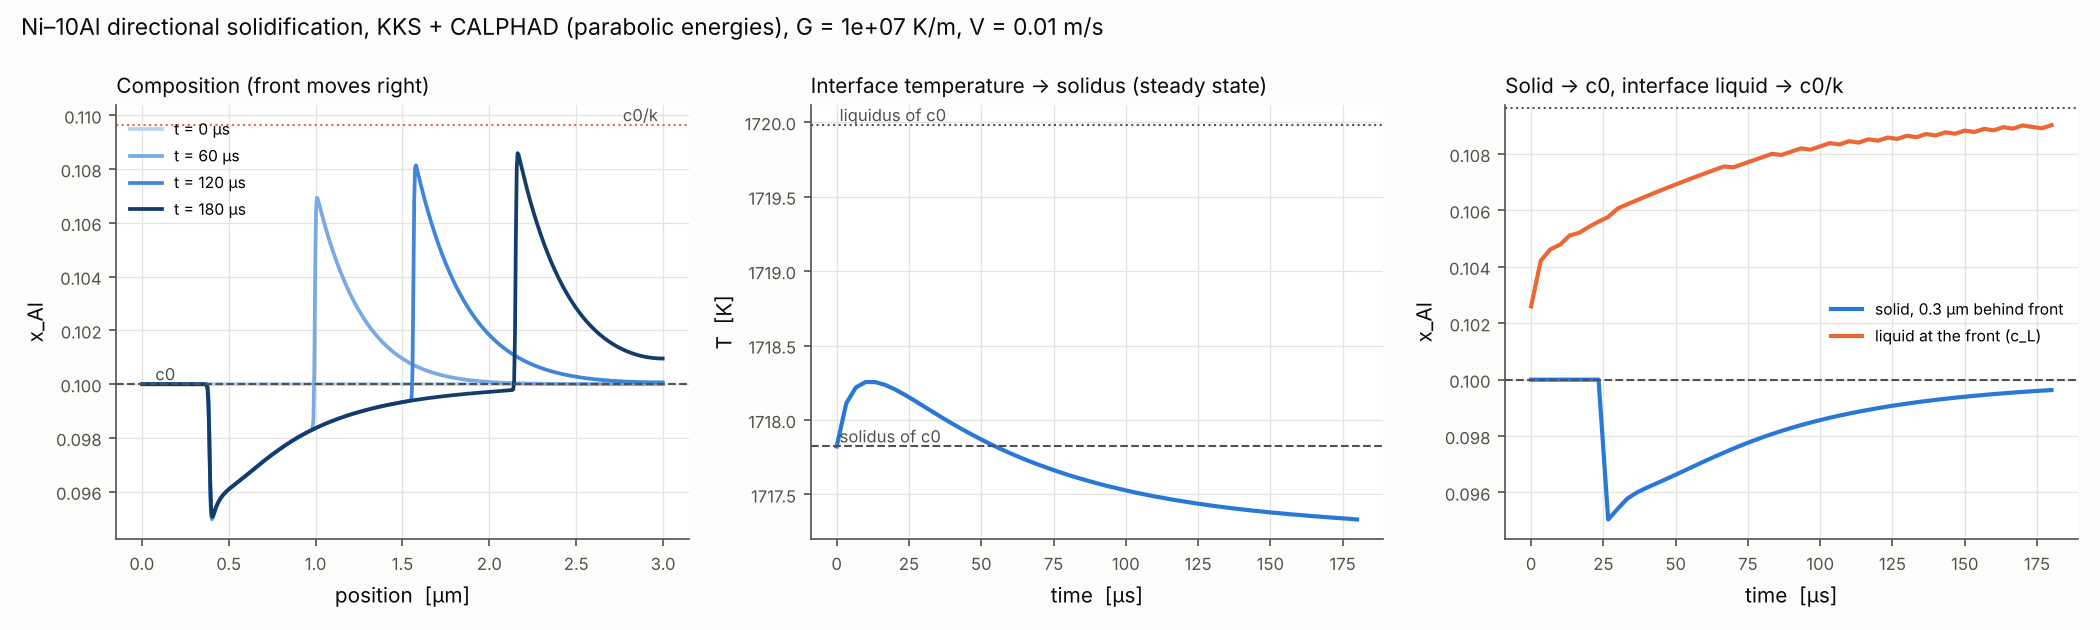
\includegraphics[width=\textwidth]{kks_1d_parabolic.png}
\caption{Ni--10Al demo output (parabolic mode): composition profiles at four times, interface temperature settling below the solidus, and solid and interface-liquid compositions approaching c0 and c0/k}
\label{fig:kks-demo}
\end{figure}

\needspace{10\baselineskip}
\section*{12. Troubleshooting, performance and limitations}
\addcontentsline{toc}{section}{12. Troubleshooting, performance and limitations}
Most problems come from a missing \texttt{db}, a phase name that differs between databases, or a phase hidden inside its ordered partner. The table maps symptoms to fixes.


\needspace{7\baselineskip}
\subsection*{Troubleshooting}
\addcontentsline{toc}{subsection}{Troubleshooting}
\begingroup\small
\begin{longtable}{>{\raggedright\arraybackslash}p{0.287\linewidth}>{\raggedright\arraybackslash}p{0.319\linewidth}>{\raggedright\arraybackslash}p{0.315\linewidth}}
\toprule
\textbf{Symptom} & \textbf{Likely cause} & \textbf{Fix} \\
\midrule
\endhead
\texttt{Several databases loaded .\allowbreak{}.\allowbreak{}.\allowbreak{}; say which with \textquotesingle{}db\textquotesingle{}.\allowbreak{}} & More than one database is loaded & Add \texttt{\textquotedbl{}db\textquotedbl{}} to the request, or set \texttt{db=} on the client \\
\texttt{Unknown phase(s) [.\allowbreak{}.\allowbreak{}.\allowbreak{}]} & Names differ between databases (\texttt{FCC\_\allowbreak{}L12} in one, \texttt{L12\_\allowbreak{}FCC} in another) & \texttt{GET /\allowbreak{}databases/\allowbreak{}\{db\}} lists the names \\
A phase you expected is missing from the results & It is reported under its ordered partner & Read \texttt{equivalent\_\allowbreak{}to}; \texttt{FCC\_\allowbreak{}L12} with \texttt{equivalent\_\allowbreak{}to: \textquotedbl{}FCC\_\allowbreak{}A1\textquotedbl{}} is \(\gamma\) \\
\texttt{stability\_\allowbreak{}check.\allowbreak{}verified} is \texttt{false} & Even 10 000 samples per phase left a positive driving force & Compare candidates with API 2, look at API 3 in points mode, or restrict \texttt{phases} \\
API 1 takes several seconds & The check re-solved with denser sampling (\texttt{sampling\_\allowbreak{}density} 2000 or 10000) & Expected for hard cases; \texttt{verify: false} skips it when certainty is not needed \\
\texttt{.\allowbreak{}.\allowbreak{}.\allowbreak{} has sublattices or vacancies mixing with the elements .\allowbreak{}.\allowbreak{}.\allowbreak{} Use mode=\textquotesingle{}table\textquotesingle{}.\allowbreak{}} & \texttt{mode=\textquotedbl{}exact\textquotedbl{}} with an ordered phase or compound & \texttt{mode=\textquotedbl{}table\textquotedbl{}} or \texttt{\textquotedbl{}parabolic\textquotedbl{}}, with \texttt{branches} for order/disorder phases \\
\texttt{mode=\textquotesingle{}parabolic\textquotesingle{} needs temperatures} & No \texttt{T} given & \texttt{T=(Tmin,\allowbreak{} Tmax,\allowbreak{} step)} or a list \\
\texttt{(.\allowbreak{}.\allowbreak{}.\allowbreak{}) never coexist in .\allowbreak{}.\allowbreak{}.\allowbreak{} K.\allowbreak{}} & The temperature range misses the two-phase field & Find the field with an API 1 sweep first \\
A tie line has \texttt{consistent: false} & The KKS energies picked a different two-phase field or branch than pycalphad & Set \texttt{c\_\allowbreak{}alloy}; set \texttt{branches} \\
\texttt{kks.\allowbreak{}warnings} mentions a kink & An order/disorder phase on the default \texttt{\textquotedbl{}lowest\textquotedbl{}} branch & \texttt{branches=\{\textquotedbl{}FCC\_\allowbreak{}L12\textquotedbl{}: \textquotedbl{}ordered\textquotedbl{}\}} \\
\texttt{split} info contains a \texttt{warning} & Newton did not converge, usually at c far from both phases & Warm-start with \texttt{ca0}, \texttt{cb0}; reduce the time step \\
\texttt{Database lacks atomic masses; use mole fractions.\allowbreak{}} & Weight units with a TDB that has no masses & Use mole fractions or atomic percent \\
C++: \texttt{calphad server unreachable} & Server not running, or wrong host or port & Start it; check \texttt{GET /\allowbreak{}health} in a browser \\
HTTP 422 & A required field is missing or has the wrong type & Compare the request with \texttt{/\allowbreak{}docs} \\
\bottomrule
\end{longtable}
\endgroup

\needspace{7\baselineskip}
\subsection*{Performance}
\addcontentsline{toc}{subsection}{Performance}
\begin{itemize}
\item Keep the server running. The first call for a new set of elements and phases compiles the models in about a second; later calls reuse them.
\item In Python, import the modules directly instead of calling the server: an HTTP round trip costs about a millisecond plus JSON encoding.
\item Never call the server per grid point. Fetch KKS parameters once, then evaluate locally.
\item Warm-start \texttt{split} with the previous step's \texttt{ca}, \texttt{cb}: 0.22 s falls to 0.06 s on a 512 \(\times\) 512 grid in exact mode. Use \texttt{parabolic} (0.03 s) for large 2-D and 3-D runs.
\item Build expensive KKS models once: \(\gamma '\) in \texttt{table} mode takes about 14 s. \texttt{export\_\allowbreak{}json} or \texttt{export\_\allowbreak{}parabolic\_\allowbreak{}csv} saves the result for later runs.
\item For energy surfaces over HTTP, prefer \texttt{step} \(\ge\) 0.01 for ternaries.
\end{itemize}
\begingroup\small
\begin{longtable}{>{\raggedright\arraybackslash}p{0.603\linewidth}>{\raggedright\arraybackslash}p{0.344\linewidth}}
\toprule
\textbf{Operation} & \textbf{Time on the test machine} \\
\midrule
\endhead
API 1, Cu--Ni, first call & 0.5 s \\
API 1, Ni--Al, six temperatures & 1.3 s \\
API 3, Al--Cr--Ni, \texttt{step} 0.05 & 0.07 s \\
\texttt{KKSModel} exact, \(\gamma\)/L & 0.04 s \\
\texttt{KKSModel} parabolic, 36 temperatures & 4.5 s \\
\texttt{KKSModel} \(\gamma '\) table, 13 temperatures & 14 s \\
1-D demo, 108 000 steps, 600 cells & 15 s parabolic, 56 s exact \\
\bottomrule
\end{longtable}
\endgroup

\needspace{7\baselineskip}
\subsection*{Limitations}
\addcontentsline{toc}{subsection}{Limitations}
\begin{itemize}
\item The KKS layer handles two phases in a binary alloy. Multicomponent or multiphase KKS is not included.
\item Anti-trapping currents and the thin-interface calibration of the mobility M are left to your solver.
\item \texttt{exact} mode handles substitutional phases only, and fixes P at 101 325 Pa.
\item The molar volume is a constant you supply; it is not read from the database.
\item The stability check catches missed phases but not every missed miscibility gap inside a phase that is already stable.
\item Only substitutional and sublattice (CEF) models were tested. Ionic liquids and other models work as far as pycalphad supports them.
\item The server has no authentication, and calls on one database run one at a time.
\item \texttt{alcrni.\allowbreak{}tdb} is a pycalphad test database, useful for exercising ordered phases but not for alloy design.
\end{itemize}

\needspace{7\baselineskip}
\subsection*{pycalphad pitfalls the framework works around}
\addcontentsline{toc}{subsection}{pycalphad pitfalls the framework works around}
\begingroup\small
\begin{longtable}{>{\raggedright\arraybackslash}p{0.343\linewidth}>{\raggedright\arraybackslash}p{0.313\linewidth}>{\raggedright\arraybackslash}p{0.265\linewidth}}
\toprule
\textbf{Pitfall} & \textbf{Seen in testing} & \textbf{What the framework does} \\
\midrule
\endhead
The minimiser stops in a local minimum when sampling misses a phase & Ni--20Al--10Cr at 1600 K: L1\(_{2}\) + liquid instead of L1\(_{2}\) + B2, 11 J/mol too high & Stability check with denser re-sampling (API 1) \\
A single ordered phase is returned in its metastable disordered state & Ni--25Al \(\gamma '\) at 1600 K, 355 J/mol too high & Multi-start minimisation (API 2, KKS tables) \\
The local driving-force search underestimates & \(\gamma '\) about 11 J/mol low & Larger of pycalphad's value and a sampled estimate \\
Disordered \(\gamma\) is named after its ordered partner & \texttt{FCC\_\allowbreak{}L12} for \(\gamma\) & \texttt{state} and \texttt{equivalent\_\allowbreak{}to} labels \\
\bottomrule
\end{longtable}
\endgroup
Tested with Python 3.13 and pycalphad 0.11.2.


\end{document}
